% !TeX encoding = latin1
%
% [ Tiedostossa käytetty merkistö on ISO 8859-1 eli Latin 1. Ylläoleva rivi ]
% [ tarvitaan, jos käyttää MiKTeX-paketin mukana tulevaa TeXworks-editoria. ]
%
% Laatinut Timo Männikkö
%
% Jos kirjoitat pro gradu -tutkielmaa, tee mallipohjaan seuraavat muutokset:
%  - Poista dokumenttiluokasta optio shortthesis .
%  - Poista makro \tyyppi .
%  - Lisää suuntautumisvaihtoehto makrolla \linja .
%  - Kirjoita ylimmän tason otsikot makrolla \chapter, toisen tason otsikot
%    makrolla \section ja mahdolliset kolmannen tason otsikot makrolla
%    \subsection .

\documentclass[finnish,nonumbib,nocopyright]{gradu2}

\usepackage{palatino} % valitaan oletusfonttia hieman tyylikkäämpi fontti

\usepackage[pdftex]{graphicx}
\usepackage{epstopdf}
\usepackage[utf8]{inputenc}

\title{Behaviour-driven development mobiiliohjelmistojen kehityksen tukena}
\translatedtitle{Using behaviour-driven development to support software development on mobile platforms}

\setauthor{Samppa}{Hynninen}
\yhteystiedot{samppa.hynninen@jyu.fi}

\setdate{04}{05}{2014}

\tiivistelma{Tähän tulee tutkielman tiivistelmä.}
\abstract{Here comes the abstract of the thesis.}

\avainsanat{bdd, behariour-driven development, mobiilialustat}    % korvaa nämä oikeilla
\keywords{bdd, behariour-driven development, mobile platforms} % avainsanoilla

\linja{Ohjelmisto- ja tietoliikennetekniikka}

\begin{document}

\mainmatter

\chapter{Johdanto}

Lähivuosina erilaisten mobiilipäätteiden osuus kuluttajien käyttämistä laitteista on kasvanut räjähdysmäisesti. Perinteisten pöytätietokoneiden, kannettavien tietokoneiden ja matkapuhelinten väliin on syntynyt täysin uusia laiteryhmiä, kuten esimerkiksi tablet-tietokoneet. Ohjelmistoteollisuus on joutunut muuntautumaan uusiin vaatimuksiin, jotka uudenlaiset sovellusalustat ovat tuoneet mukanaan. Palvelujen tulee nykyään monesti olla käytettävissä useilla eri alustoilla ja erilaisia alustoja voivat koskea erilaiset vaatimukset. Ohjelmistokehitysmenetelmiä on jouduttu kehittämään jatkuvasti muuttuvan ympäristön ja uusien tarpeiden myötä. Behaviour-driven development, eli käyttäytymislähtöinen kehitys on yksi viime vuosina kehittyneistä ohjelmistokehitystä tukevista tekniikoista, jossa kehityksen lähtökohtana ovat määrittelyt siitä, kuinka ohjelmiston tulisi toimia ja käyttäytyä.

Ohjelmistotestauksen ollessa kriittinen osa ohjelmistotuotantoprosessia ja erityisesti laadunvarmistusta, sen merkitys korostuu entisestään, kun ohjelmistoja toimitetaan useille eri alustoille. Tässä tutkielmassa käsitellään behaviour-driven developmentia ja sen taustoja niin menetelmällisestä kuin puhtaasti teknologisesta näkökulmasta. Aluksi selvitetään mitä BDD:llä tarkoitetaan ja mistä se on kehittynyt. Taustojen ja historian ohella katselmoidaan ohjelmistokehityksen haasteita ja ongelmakohtia, joita BDD:n avulla pyritään välttämään. Teknologioiden osalta käsitellään erityisesti BDD-testaamista mobiiliohjelmistojen kehityksessä ja sen poikkeavuuksia sekä erityispiirteitä verrattuna BDD-menetelmiin muissa ympäristöissä. Tässä yhteydessä tarkastellaan erikseen eri mobiilialustojen natiivisovelluksia sekä uusiin HTML5-teknologioihin pohjautuvia alustariippumattomia sovelluksia, sillä niiden testaaminen eroaa merkittävästi toisistaan. 

Tämän pro gradu -tutkielman tavoitteena on kartoittaa behaviour-driven developmentin tarjoamia mahdollisuuksia helpottaa mobiiliohjelmistojen kehitystä ja erityisesti testausta. Tarkoituksena on selvittää millaisia BDD-testikehyksiä merkittävimmille mobiilialustoille on tällä hetkellä olemassa ja miten eri mobiilialustojen testikehykset poikkeavat toisistaan. Tämä lisäksi tarkoituksena on selvittää, millaisia liiketoiminnallisia etuja BDD:llä voidaan mobiilisovelluskehityksessä saavuttaa. Tutkielma toteutetaan käyttäen konstruktiivista tutkimusotetta ja siinä pyritään lopputuloksena toteuttamaan ympäristö, jossa samaa sovellusta voitaisiin testataan eri mobiilialustoilla yhdellä testikokoelmalla. Testiympäristön toteutuksen yhteydessä tutkitaan millaisia puutteita nykyratkaisuissa on ja miten niitä voitaisiin kehittää, jotta yhden testikokoelman mallia voitaisiin käyttää.

\section{Termejä}
\begin{itemize}
\item Apache Cordova: Avoimen lähdekoodin ohjelmisto, johon PhoneGap perustuu.
\item ATDD: Acceptance test-driven development. Hyväksymistestilähtöinen ohjelmistokehitys.
\item BDD: Behaviour-driven development. Käyttäytymislähtöinen kehitys. Ohjelmistokehitysprosessi, jossa vaatimukset pohjautuvat ohjelmiston käyttäytymiseen.
\item CI: Continuous Integration, jatkuva integraatio.
\item Cucumber: Rubylla kirjoitettu BDD-testikehys.
\item HTML5: HTML-merkintäkielen uusin versio ja samalla käsite nykyaikaisille web-teknologioille, kuten JavaScriptille ja CSS3:lle.
\item Jasmine: BDD-testikehys JavaScript-ohjelmointikielelle.
\item JBehave: Yksi ensimmäisistä BDD-testikehyksistä Java-ohjelmointikielelle.
\item Natiivisovellus: Jonkin sovellusalustan omalla kehitysympäristöllä ja ohjelmointikielellä toteutettu sovellus.
\item PhoneGap: Adoben omistama mobiiliohjelmistokehys, jolla voidaan toteuttaa monialustaisia sovelluksia moderneilla web-teknologioilla.
\item RSpec: BDD-testikehys Ruby-ohjelmointikielelle.
\item Selenium: Työkalu verkkoselaimen automatisointiin.
\item TDD: Test-driven development. Testivetoinen kehitys, ohjelmistokehityksen prosessi, jossa testit kirjoitetaan ennen ohjelmakoodia
\end{itemize}

\section{Tutkimusmenetelmistä}
Tutkimus on toteutettu käyttäen konstruktiivista tutkimusotetta. Konstruktiivisessa tutkimusotteessa tavoitteena on rakentaa jonkinlainen artefakti, joka ratkaisee jonkin tietyn alan kysymyksen ja tätä kautta lisää tietoa ongelmasta ja sen ratkaisusta alalla \cite{constructive}. Tutkielmassani yritän löytää ratkaisua kysymykseen, voidaanko tämänhetkisten modernien mobiilialustojen ohjelmistoja testata tehokkaasti käyttäen Behaviour-driven developmentin toimintatapoja.

Tutkimuskysymykseen vastatakseni tutkimuksessa kartoitetaan ensiksi millaisia BDD-työkaluja mobiilialustoille on nykyään saatavilla. Tutkimuksessani käytettävät alustat olen rajannut kattamaan kolme suosituinta alustaa Gartnerin tutkimuksen pohjalta (Q4/2013) \cite{marketshare}. Kolme mukaan otettua alustaa olivat Googlen Android, Applen iOS ja Microsoftin Windows Phone. Tämän jälkeen tehtävänä oli kartoittaa valituille alustoille tällä hetkellä olemassa olevia BDD:n mahdollistavia ratkaisuja. Löydettyjä ratkaisuja käydään läpi luvussa \ref{chap:platforms}.

Olemassa olevien ratkaisuiden kartoittamisen myötä tutkielmassa tutkittiin onko mahdollisesti jo olemassa BDD-testikehyksiä, joilla voidaan testata kerralla useita eri alustoja. Samalla tutkittiin onko eri mobiilialustoille löydettävissä sellaisia BDD-testikehyksiä, joiden käyttämä luonnollinen kieli toimisi niin, että samoilla luonnollisella kielellä kirjoitetuilla testeillä voisi ainoastaan eri testikehysten kieltä jäsentävää ohjelmakoodia muokkaamalla saada samat testit toimimaan eri testikehyksillä.

Tämän jälkeen tutkimuksessa käydään vielä läpi erikseen ratkaisu ongelmaan, kun kyseessä ovat natiivisovellusten sijaan HTML5-sovellukset, sillä näiden kohdalla testaus voidaan suorittaa eri tavalla. Tutkimuksessa kartoitetaan HTML5-sovellusten testaamista sekä käydään läpi ratkaisuja, joilla HTML5-sovelluksia voidaan paketoida helposti eri alustoja varten ja näin ollen saavuttaa samat edut BDD:llä kuin natiivisovellusten kohdalla. Tästä muodostetaan oma ratkaisunsa täydentämään natiivisovellusten testaukseen löytyneitä ratkaisuja.

\chapter{Kirjallisuuskatsaus}

\section{Aikaisemmat tutkimukset}
Aikaisempaa tieteellistä tutkimusta Behaviour-driven developmentista on tehty verrattain vähän, sillä aihepiiri on niin tuore. Terminä BDD on tullut käyttöön ensimmäisiä kertoja vasta 2000-luvun puolivälissä erirtyisesti Dan Northin blogitekstien myötä \cite{bddintro}. Täten voidaan laskea BDD:n olevan käsitteenäkin vasta noin kymmenen vuoden ikäinen.

Hakiessani lähteitä ja aikaisempia tutkimuksia BDD:n aihepiireistä käytin pääasiallisesti suurimpia tietokantoja etsimiseen. Näitä olivat ACM Digital Library, IEEE Xplore, Google Scholar. Aloitin haut tekemällä muutamia avainsanahakuja \cite{tutkimuspaska} eri tietokantoihin. Termillä ``bdd'' tehdyt haut eivät tuottaneet juuri mistään kannasta toivottuja tuloksia, sillä lyhennettä ilmeisesti käytetään monilla muillakin tieteenaloilla tarkoittamaan eri asiaa. Avainsanahaussa hakusanat ``behaviour driven development'' tuottivat jo selvästi paremman tuloksen. Google Scholar palautti kyselyllä noin 250 tulosta, joista suuri osa oli relevantteja. IEEE Xploresta ei samoilla hakutermeillä ja sen variaatioilla palautunut kuin kaksi eri julkaisua. ACM:n hausta termeillä ja niiden muutamalla variaatiolla (esim. ``behavior driven development'') palautui noin kaksikymmentä tulosta.

Hauilla löytyneet tutkimukset pystyi karkeasti jakamaan muutamaan eri luokkaan. Ensimmäiseen ryhmään kuuluvissa tutkimuksissa keskityttiin lähinnä määrittelemään Behaviour-driven developmentia ja ylipäänsä siihen liittyvää termistöä. Näissä tutkimuksissa ja lähteissä aihepiiri oli ikäänkuin uusi ja vielä vakiintumaton. Toisen pääteeman löytyneissä tutkimuksissa muodostavat lähteet, joissa BDD:n tehokkuutta ja sopivuutta on tutkittu eri tilanteissa. Tähän teemaan lukeutuvat myös tutkimukset, joissa BDD:n menetelmiä sovelletaan jollekin tietylle toimialalle.

Sopivimmille artikkeleille tein lisähakuja käyttäen ``Backward search''-menetelmää \cite{tutkimuspaska}, jossa kävin läpi löytyneiden tutkimusten lähteitä. Tällä tavoin löytyi muutamia lähteitä, jotka esiintyivät hyvin monissa BDD:hen liittyvissä tutkimuksissa. Näitä olivat esimerkiksi Dan Northin tekstit \cite{bddintro}, Gojko Adzicin kirjat \cite{bridging},\cite{specification} sekä esimerkiksi Cucumber-kirja \cite{cucumber}. Samanlaisia tuloksia löytyi, kun kävin lähteille läpi vielä ``Backward search''-menetelmää, mutta tällä kertaa keskittyen kirjoittajiin, eli tutkin kirjoittajien muita teoksia.

Näiden hakujen myötä päädyin käyttämään lähteinä erityisesti usein esilletulleita teoksia, kuten Adzicin kirjat, Cucumber-kirja sekä Dan Northin kirjoitukset. Tämän lisäksi mukaan valikoitui kirjoittaessa jatkuvasti uusia lähteitä, joita löytyi ennen kaikkea tekemällä ``Backward search''-hakuja aineistolle.

\chapter{Ketterä ohjelmistokehitys}

\section{Taustaa ja ketterien menetelmien kehitys}

Niin kauan kuin tietokoneohjelmistoja on kehitetty, on niiden yhteydessä kehitetty myös erilaisia malleja, joiden tarkoituksena on helpottaa ja sujuvoittaa ohjelmistokehitystä. Menetelmät voidaan karkeasti jakaa inkrementaalisiin ja iteratiivisiin menetelmiin \cite{iterative}. Inkrementaalisissa malleissa ideana on se, että ohjelmisto kasvaa jatkuvasti kehittyen kohti lopullista valmista tuotetta, kun taas iteratiivisissa malleissa ohjelmistoa kehitetään pienissä osissa lyhyemillä aikaväleillä ja tätä työtä toistetaan useaan otteeseen. Seuraavassa esitelläänkin muutamia tunnettuja ohjelmistotuotannon malleja ja niiden kehitystä kohti ketteriä menetelmiä.

\subsection{Vesiputousmalli}

Yksi varhaisista ohjelmistokehityksen malleista on inkrementaalinen vesiputousmalli, jonka perustana toimii hyvin pitkälti Winston Roycen kuvaama malli artikkelissaan Managing the development of large software systems \cite{managing} vuodelta 1970. Huolimatta siitä, että vesiputousmalli on erittäin vanha ja sen käyttäminen sisältää tunnettuja riskejä, on malli edelleen hyvin suosittu. Roycen malli perustuu ajatukselle, että kaikissa ohjelmistokehitystehtävissä on aina ainakin kaksi vaihetta, analyysivaihe ja itse ohjelmiston koodausvaihe. Vesiputousmallissa luodaan tämän ajatuksen ympärille laajempi malli, jossa edellämainittuja vaiheita on täydennetty uusilla vaiheilla, jotka ovat kuitenkin täysin erillisiä analyysi- ja koodausvaiheista. Näitä ovat Roycen mallissa \cite{managing} kaksi vaatimusmäärittelyvaihetta, ohjelmiston suunnittelu ja koodauksen jälkeinen testausvaihe. Näillä lisäyksillä malli on soveltuvampi suurten ohjelmistoprojektien läpivientiin. Roycen esittämä malli ei kuitenkaan ole täysin se vesiputousmalli, joka on vielä nykyäänkin käytössä, sillä Royce itsekin ehdottaa parhaimpana versiona mallistaan sellaista, jossa eri vaiheiden välillä voidaan liikkua kumpaankin suuntaan, eli myös takaisinpäin edellseen vaiheeseen.

Royce kuitenkin tiedostaa vesiputousmallin sisältämiä riskejä jo omassa artikkelissaan. Yksi näistä on esimerkiksi vaara, että vasta testivaiheessa huomataan puutteita, jotka johtavat perinpohjaisiin muutoksiin ohjelmiston rakenteessa tai toiminnassa, jolloin käytännössä koko kehitysprosessi joudutaan aloittamaan alusta. Näitä puutteita voi suurellakin todennäköisyydellä ilmetä, sillä testausvaihe on ensimmäinen kerta, kun järjestelmä toimii kokonaisuutena integroituna muihin järjestelmiin \cite{managing}. Toinen merkittävä tekijä, joka monesti jätetään huomioimatta vesiputousmallia käytettäessä, on se, että Royce itsekin suosittelee käymään prosessin läpi kahteen kertaan. Tämä pätee etenkin tilanteisiin, jossa toimitetaan asiakkaalle jokin täysin uusi tuote. Tällöin ensimmäisellä kerralla luodaan pilotti tuotteesta lyhyessä ajassa. Tämän pilotin tarkoituksena on tuoda esiin kehitettävän tuotteen erityiset haasteet, löytää suunnittelun mahdolliset puutteet sekä luoda eri vaihtoehtoja näiden ratkaisemiseen \cite{managing}. Tällöin lyhyessä ajassa kehitetty pilottituote toimii ikään kuin koko projektin simulaationa, jolloin vaikeisiin tilanteisiin osataan varautua paremmin.

Royce ei itsekään pitänyt malliaan parhaana mahdollisena suurten ohjelmistojen kehitykseen, vaan Larmanin ja Basilin artikkelissa \cite{iterative} kerrotaankin, kuinka hän itsekin toteaa vesiputousmallin olevan kaikista yksinkertaisin malli, joka ei kuitenkaan todennäköisesti tule toimimaan kuin kaikkein yksinkertaisimpien ja suoraviivaisimpien projektien yhteydessä. Ensimmäiset maininnat ja kehotukset iteratiiviseen ohjelmistokehitykseen ovatkin jo ajalta ennen Roycen mallin julkaisua. Jo vuonna 1969 IBM:n tutkimuskeskuksessa M.M Lehman kuvasi iteratiivista mallia, jossa erotettiin suunnittelu, arviointi ja dokumentointi \cite{iterative}. Tässä mallissa suunnittelu tuotti jo toimivan mallin, jota sitten iteratiivisesti kehitettiin eteenpäin.

Kuitenkin vielä nykypäivänäkin suuriakin ohjelmistoprojekteja toteutetaan käyttäen vesiputousmallia, sillä sen koetaan sisältävän joitain etuja tietyissä ohjelmistoprojektin vaiheissa verrattuna ketteriin menetelmiin. Monesti nämä ratkaisevat edut liittyvät erityisesti projektien myyntiin tarjousvaiheessa tehtyjen tarjousten muotoiluun. Vesiputousmallilla myytävissä ratkaisuissa on helpompaa myydä asiakkaalle kiinteällä hinnalla yksi tarkasti määritelty kokonaisuus, jonka myötä asiakas kokee tietävänsä tarkalleen, millaisen tuotteen hän on saamassa ja mihin hintaan. Ketteriä projekteja myytäessä asiakas käytännössä ostaa vain työtä, eikä kiinteästi määritettyä lopputulosta \cite{valtiokonttori}. Tällöin asiakkaalle jää jatkuvasti mahdollisuus vaikuttaa siihen, että tehty työ on juuri sitä, mistä hänelle on eniten hyötyä, eikä ohjelmistoon toteuteta esimerkiksi täysin turhia tai vanhentuneita vaatimuksia. Kuitenkin tästä huolimatta monesti ainoastaan lopullinen kiinteä hinta ja myyntivaiheessa määritelty lopputulos ratkaisevat ostopäätöstä tehdessä, jolloin edelleen nykyään saatetaan päätyä toteuttamaan projekteja vesiputousmallia käyttäen.

\begin{figure}
\centering
\includegraphics[width=0.95\textwidth]{vesiputous}
\caption{Vesiputousmalli \cite{managing}}
\end{figure}

\subsection{Spiraalimalli}

Spiraalimalli on Barry Boehmin kehittämä \cite{spiral} malli vuodelta 1986, joka on ensimmäisiä tunnettuja iteratiivisia malleja ohjelmistokehityksessä. Spiraalimallin tärkeimpänä ajatuksena on se, että siinä otetaan riskit entistä paremmin huomioon verrattuna esimerkiksi perinteiseen vesiputousmalliin. Spiraalimallissa jokainen iteraatio sisältää neljä merkittävää osaa, jotka ovat \cite{spiral}:
\begin{enumerate}
\item Iteraation tavoitteiden, vaihtoehtojen ja rajoitteiden määrittely
\item Eri vaihtoehtojen arviointi sekä riskien tunnistaminen ja arviointi
\item Kehitystyö ja seuraavan tason tuotteen määrittely
\item Seuraavan iteraation suunnittelu
\end{enumerate}

\begin{figure}
\centering
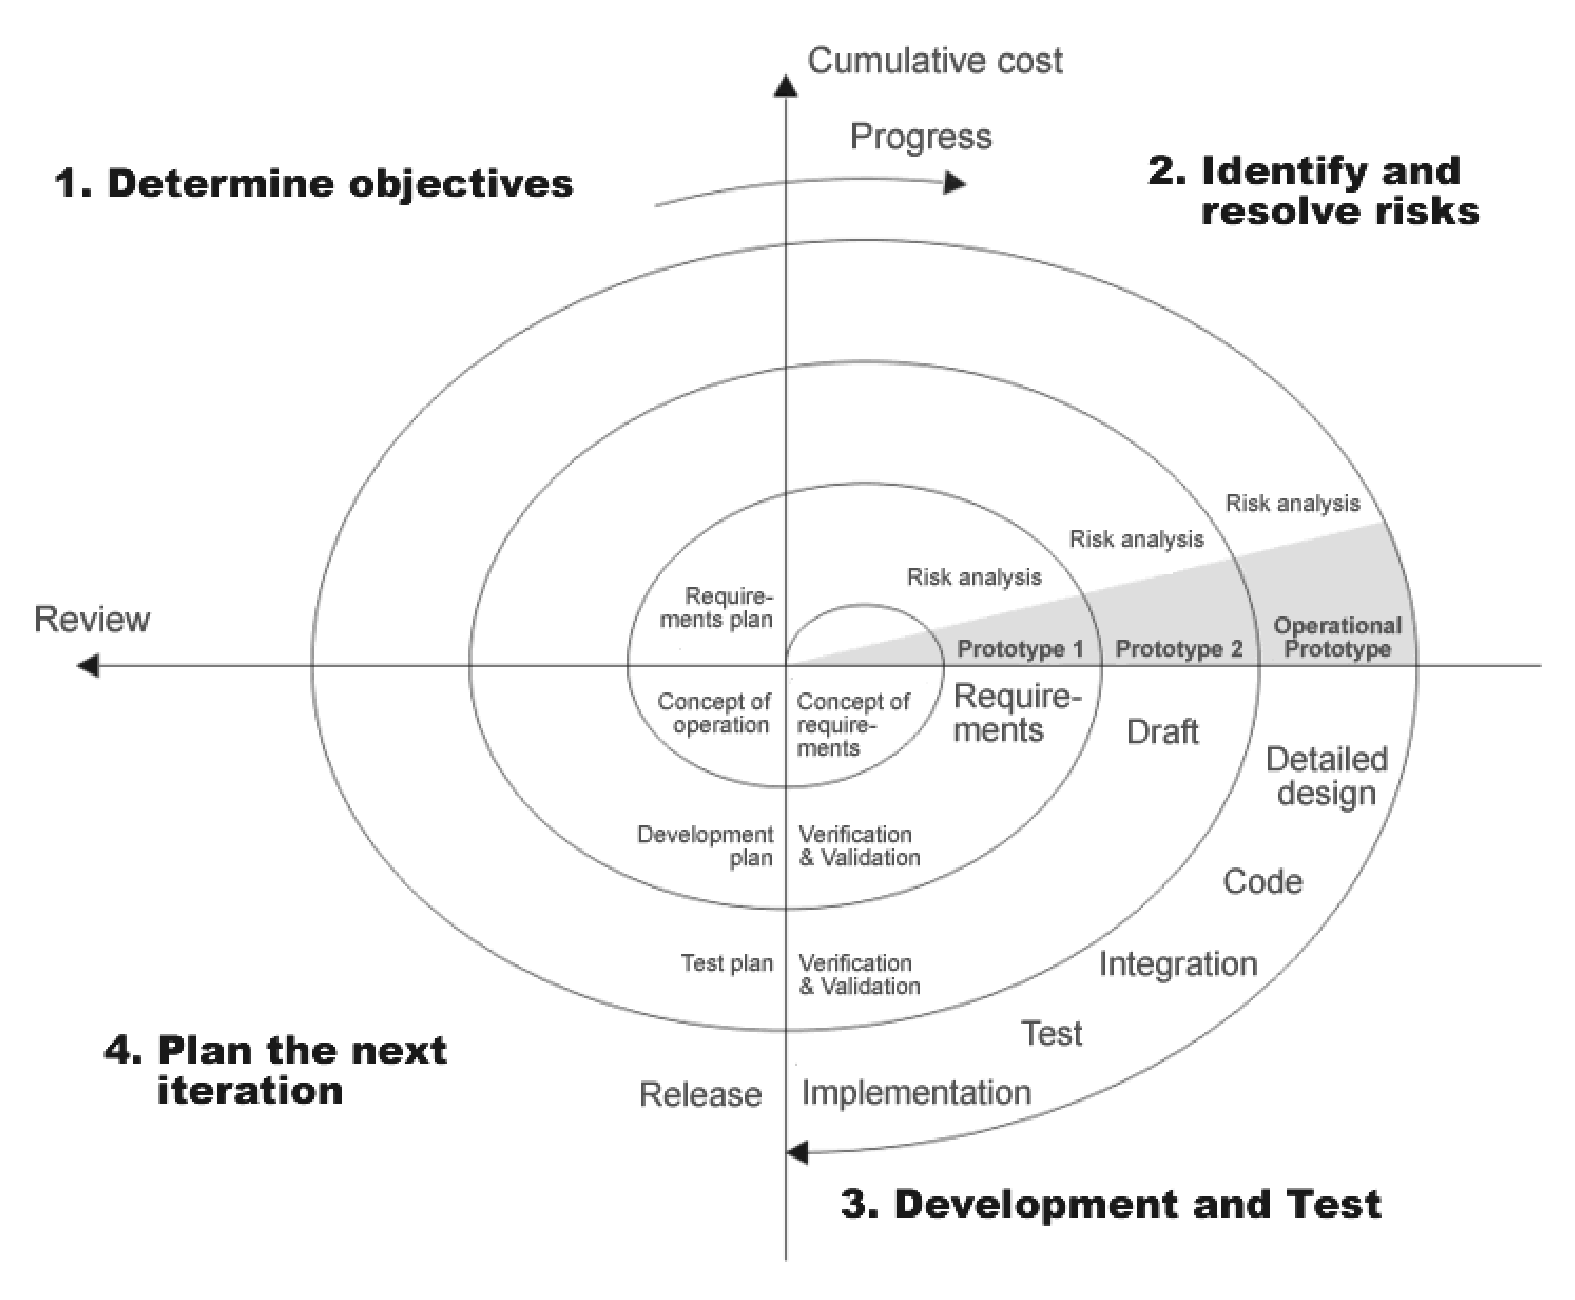
\includegraphics[width=1.00\textwidth]{spiral}
\caption{Spiraalimalli \cite{managing}}
\end{figure}

Mallissa jokaisessa iteraatiossa toteutetaan riskianalyysin jälkeen prototyyppimalli, josta sitten lähdetään kehittämään valmista tuotetta, aivan kuten Roycen \cite{managing} ehdottamassa pilottituotemallissa. Lisäksi spiraalimallissa merkittävää on se, että jokainen iteraatiokierros sillä hetkellä valmiina olevan tuotteen arviointiin, johon osallistuvat kaikki tärkeimmät henkilöt, jotka tulevat käyttämään tuotetta \cite{spiral}. Boehmin malli toimiikin pohjana hyvin monille nykyisille ketterille menetelmille, joissa hyödynnetään samankaltaisia iteraatioita. Esimerkiksi seuraavana käsiteltävässä Scrumissa sprintit vastaavat hyvin pitkälle spiraalimallin iteraatioita, eli Scrum käytännössä sisältää spiraalimallin prosessit, joiden päälle on vielä vain lisätty muuta.

Spiraalimallissa käytetään erittäin paljon riskiä määrittämään tehtäviä asioita. Boehmin mukaan \cite{spiral} esimerkiksi eri työvaiheisiin käytettävä aika määräytyy sen perusteella, miten ne vaikuttavat olemassaolevaan riskiin. Jos esimerkiksi testaukseen käytetty aika pienentää projektin kokonaisriskiä, siihen kannattaa käyttää aikaa mieluummin kuin esimerkiksi uuden sovelluskehyksen käyttöön vanhan tutun sovelluskehyksen sijaan, sillä tällainen valinta vain lisäisi projektin riskiä ja epäonnistumisen mahdollisuutta. Tämän lisäksi Boehmin mukaan projektiryhmä käyttää riskin arviointia siihen, kuinka yksityiskohtaisella tasolla asioita kannattaa projektissa tehdä \cite{spiral}. Esimerkiksi projektin dokumentointi voisi olla yksi osa-alue, johon tätä voidaan soveltaa. Projektiryhmän tulee tällöin tehdä päätös, milloin projektin dokumentaatio on riittävällä tasolla siten, että sen tarkentamisesta ja edelleen kehittämisestä ei saada enää mitään hyötyä, vaan se voi johtaa vain kasvavaan riskiin, kuten esimerkiksi julkaisun myöhästymiseen.

Uudemmassa julkaisussaan vuodelta 2000 Boehm \cite{spiral2} vielä erikseen listaa merkkejä, jotka erottavat projektin spiraalimallista ja ovat ennenkaikkea haitallisia projektin onnistumisen edellytyksille. Käytännössä nämä merkit ovat sellaisia, joista voidaan huomata käytettävän oikeasti vesiputousmallia, jota vain nimitetään spiraalimalliksi. Tällaisia merkkejä ovat Boehmin mukaan seuraavat kuusi olettamusta \cite{spiral2}:
\begin{enumerate}
\item Vaatimukset tunnetaan ennen ohjelmiston toteutusta
\item Vaatimuksissa ei ole epäselviä olettamuksia
\item Vaatimusten luonne ei muutu kehitystyön ja projektin etenemisen myötä
\item Vaatimukset täyttävät kaikkien sidosryhmien edustajien oletukset
\item Oikea arkkitehtuuri vaatimusten täyttämiseen on hyvin ymmärretty ja omaksuttu
\item Tarpeeksi kalenteriaikaa on varattu, jotta voidaan edetä peräkkäisessä järjestyksessä vaihe kerrallaan
\end{enumerate}

Boehm määrittelee myös erilaisia invariantteja, jotka tulee olla olemassa spiraalimallin toimimisen edellytyksenä \cite{spiral2}. Nämä invariantit käytännössä määrittelevät vain tarkemmin spiraalimallin eri osa-alueet ja niiden sisällöt. Näihin Boehmin invariantteihin kuuluu esimerkiksi edellämainitut käytettävän panoksen määrittely riskin perusteella sekä työvaiheen toteutuksen yksityiskohtaisuuden tason arviointi riskin perusteella. Näiden lisäksi Boehmin määrittelemiin invariantteihin lasketaan myös keskittyminen järjestelmään ja sen elinkaareen sen sijaan, että ainoastaan mietittäisiin ohjelmiston kehittämistä teknisestä näkökulmasta \cite{spiral2}.

\subsection{Scrum}

Scrum on moderni iteratiivinen ohjelmistokehityksen viitekehys, jota ovat kehittäneet pääasiallisesti yhdysvaltalaiset Ken Schwaber ja Jeff Sutherland aina 1990-luvun alkupuolelta lähtien. Kuten termi viitekehys antaa ymmärtää, ei Scrum tarjoa mitään yksityiskohtaista prosessia ohjelmistoprojektin toteuttamiseen, vaan ennemminkin juuri kehyksen, jonka puitteissa voidaan hallita monimutkaisten tuotteiden kehitystä \cite{scrumguide}. Scrum tarjoaa käytännön työkalut ohjelmistojen kehittämiseen iteratiivisesti siten, että riski on jatkuvasti mahdollisimman pieni ja työn tulokset optimoituja, eli käytännössä tehdään aina sitä, mikä on juuri sillä hetkellä asiakkaalle kaikkein hyödyllisintä. Tämä saavutetaan, kun työskennellään nojautuen Scrumin kolmeen lähtökohtaan, jotka ovat läpinäkyvyys, tarkastelu ja sopeutuminen \cite{scrumguide}.

Läpinäkyvyys tulee Scrumissa ilmi erityisesti esimerkiksi siinä, että kaikki eri sidosryhmät ovat jatkuvasti tietoisia toteutettavan projektin tilanteesta. Käytännön työssä tämä on toteutettu monin eri tavoin \cite{scrumguide}:

\begin{itemize}
\item Työtä suoritetaan kiinteän pituisissa jaksoissa, joita kutsutaan sprinteiksi. Usein sprinttien kesto on yhdestä kolmeen viikkoa. Näihin sprintteihin projektitiimi ottaa mukaan työtä niin paljon kuin he arvioivat kykenevänsä toteuttamaan. Tässä kohtaa ainoastaan projektitiimi voi määritellä mitä he tekevät, sillä heillä on ainoina henkilöinä tieto siitä, mitä he tiiminä pystyvät toteuttamaan. Tämä sprintiin otettu työ muodostaa sprintin backlogin, johon voidaan sprintin suunnittelun jälkeen ainoastaan projektitiimin luvalla ottaa lisää työtä. Tällöin asiakas ja projektin muut sidosryhmät tietävät aina mitä seuraavan sprintin aikana on tarkoituksena saada toteutetuksi \cite{scrumguide}.
\item Koko projektin seurantaan ja läpinäkyvyyteen Scrumissa on olemassa tuotteen backlog, joka sisältää kaikki tulevaisuudessa toteutettavaksi toivotut ominaisuudet ja tehtävät asiakkaan puolelta. Tätä tuotebacklogia asiakas priorisoi yhdessä Scrum-tiimiin kuuluvan tuoteomistajan kanssa. Tämä tarkoittaa sitä, että backlogilla nostetaan prioriteetiltaan tärkeimmät tehtävät ensimmäisiksi. Tämä on tärkeää, sillä projektitiimi ottaa sitten tuotebacklogilta jokaiseen sprintiin niin paljon työtä kuin he kokevat pystyvänsä tekemään. Työtä otetaan tuotebacklogilta mukaan sprintiin siinä järjestyksessä, mihin asiakas on tehtävät yhdessä tuoteomistajan kanssa priorisoinut.
\item Projektissa toteutettavan tuotteen tila on koko ajan selvillä kaikille sidosryhmille, sillä Scrumissa on tavoitteena, että jokaisen valmiin sprintin jälkeen projektiryhmä voisi toimittaa asiakkaalle käytännössä toimivan inkrementin toteutettavaan ohjelmistoon, jolloin jokaisen sprintin työn tulos olisi heti nähtävillä. Käytännössä toimivan inkrementin toimitus ei kuitenkaan aina ole esimerkiksi projektin luonteen vuoksi mahdollista, jos toteutettavana tuotteena on jokin laaja tietojärjestelmä, jossa käytetään useita sprinttejä esimerkiksi pelkästään back endin tai tietokantojen toteuttamiseen. Tällöin inkrementti voi olla kuitenkin toimiva, vaikkei asiakas siitä heti suoraa hyötyä saisikaan.
\end{itemize}

Tehtyä työtä, työtapoja ja projektia kokonaisuudessa arvioidaan ja tarkastellaan Scrumin puitteissa jatkuvasti. Erityistä tässä on se, että näitä asioita ei ole arvioimassa vain yksi taho, vaan työn ja tulosten tarkastelua tehdään jatkuvasti kaikkien toimesta, jotka liittyvät projektiin millään tapaa.

Päivittäin työtä arvioidaan ns. daily-palavereissa, joissa jokainen projektitiimin jäsen pääsee kertomaan mitä on tehnyt, mitä aikoo tehdä ja samalla hän voi kertoa, jos työssä on ilmennyt jotain ongelmia. Tällaisen lyhyen kiinteästi 15-minuuttiseksi ajoitetun palaverin myötä koko tiimi on joka päivä selvillä siitä, mitä muut tekevät ja mahdollisesti pystyvät näin ollen esimerkiksi auttamaan muita ja tehostamaan omaa työtään sillä, etteivät he tee päällekkäisiä tai toisistaan riippuvia tehtäviä.

Jokaisen sprintin päättyessä järjestetään niin kutsuttu sprintin arviointi, jossa projektitiimi yhdessä asiakkaan kanssa käy product ownerin johdolla läpi sprintin aikana toteutettuja ominaisuuksia ja tehtäviä. Samassa tilaisuudessa käydään läpi ne sprintiin mukaan otetut työt, joita projektitiimi ei ole ehtinyt saada valmiiksi. Sprintin arviointi onkin hyvä tilaisuus sekä projektitiimille, että asiakkaalle, sillä tällöin kummatkin pääsevät yhdessä keskustelemaan siitä, mitä tiimi on tehnyt. Tällöin asiakkaalla on mahdollisuus esittää kysymyksiä ja toteuttava tiimi pääsee myös kertomaan mahdollisista ongelmista ja niiden ratkaisuista, eli tilaisuudessa pystytään viimeistään oikomaan mahdollisia väärinkäsityksiä tai näkemyseroja.

Daily-palaverien ja sprintin arvioinnin lisäksi projektitiimi käy jokaisen sprintin jälkeen läpi retrospektiivin, jossa jokaisella tiimin jäsenellä on mahdollisuus arvioida, mikä tiimin työssä meni hyvin ja millä alueilla on vielä kehitettävää. Nämä onnistumiset liittyvät yleensä ennemminkin tiimin sisäisiin asioihin kuin mihinkään muuhun, eli ennenkaikkea asioihin, joihin tiimi itse voi vaikuttaa. Tällaisia asioita ovat esimerkiksi:
\begin{itemize}
\item Kuinka hyvin Scrumin periaatteita on noudatettu?
\item Onko tiimin sisäisessä dynamiikassa jotain ongelmia?
\item Voisiko työtapoja parantaa jotenkin?
\item Onko jotain projektiin liittymättömiä ongelmia, jotka haittaavat työtä?
\end{itemize}

\begin{figure}
\centering
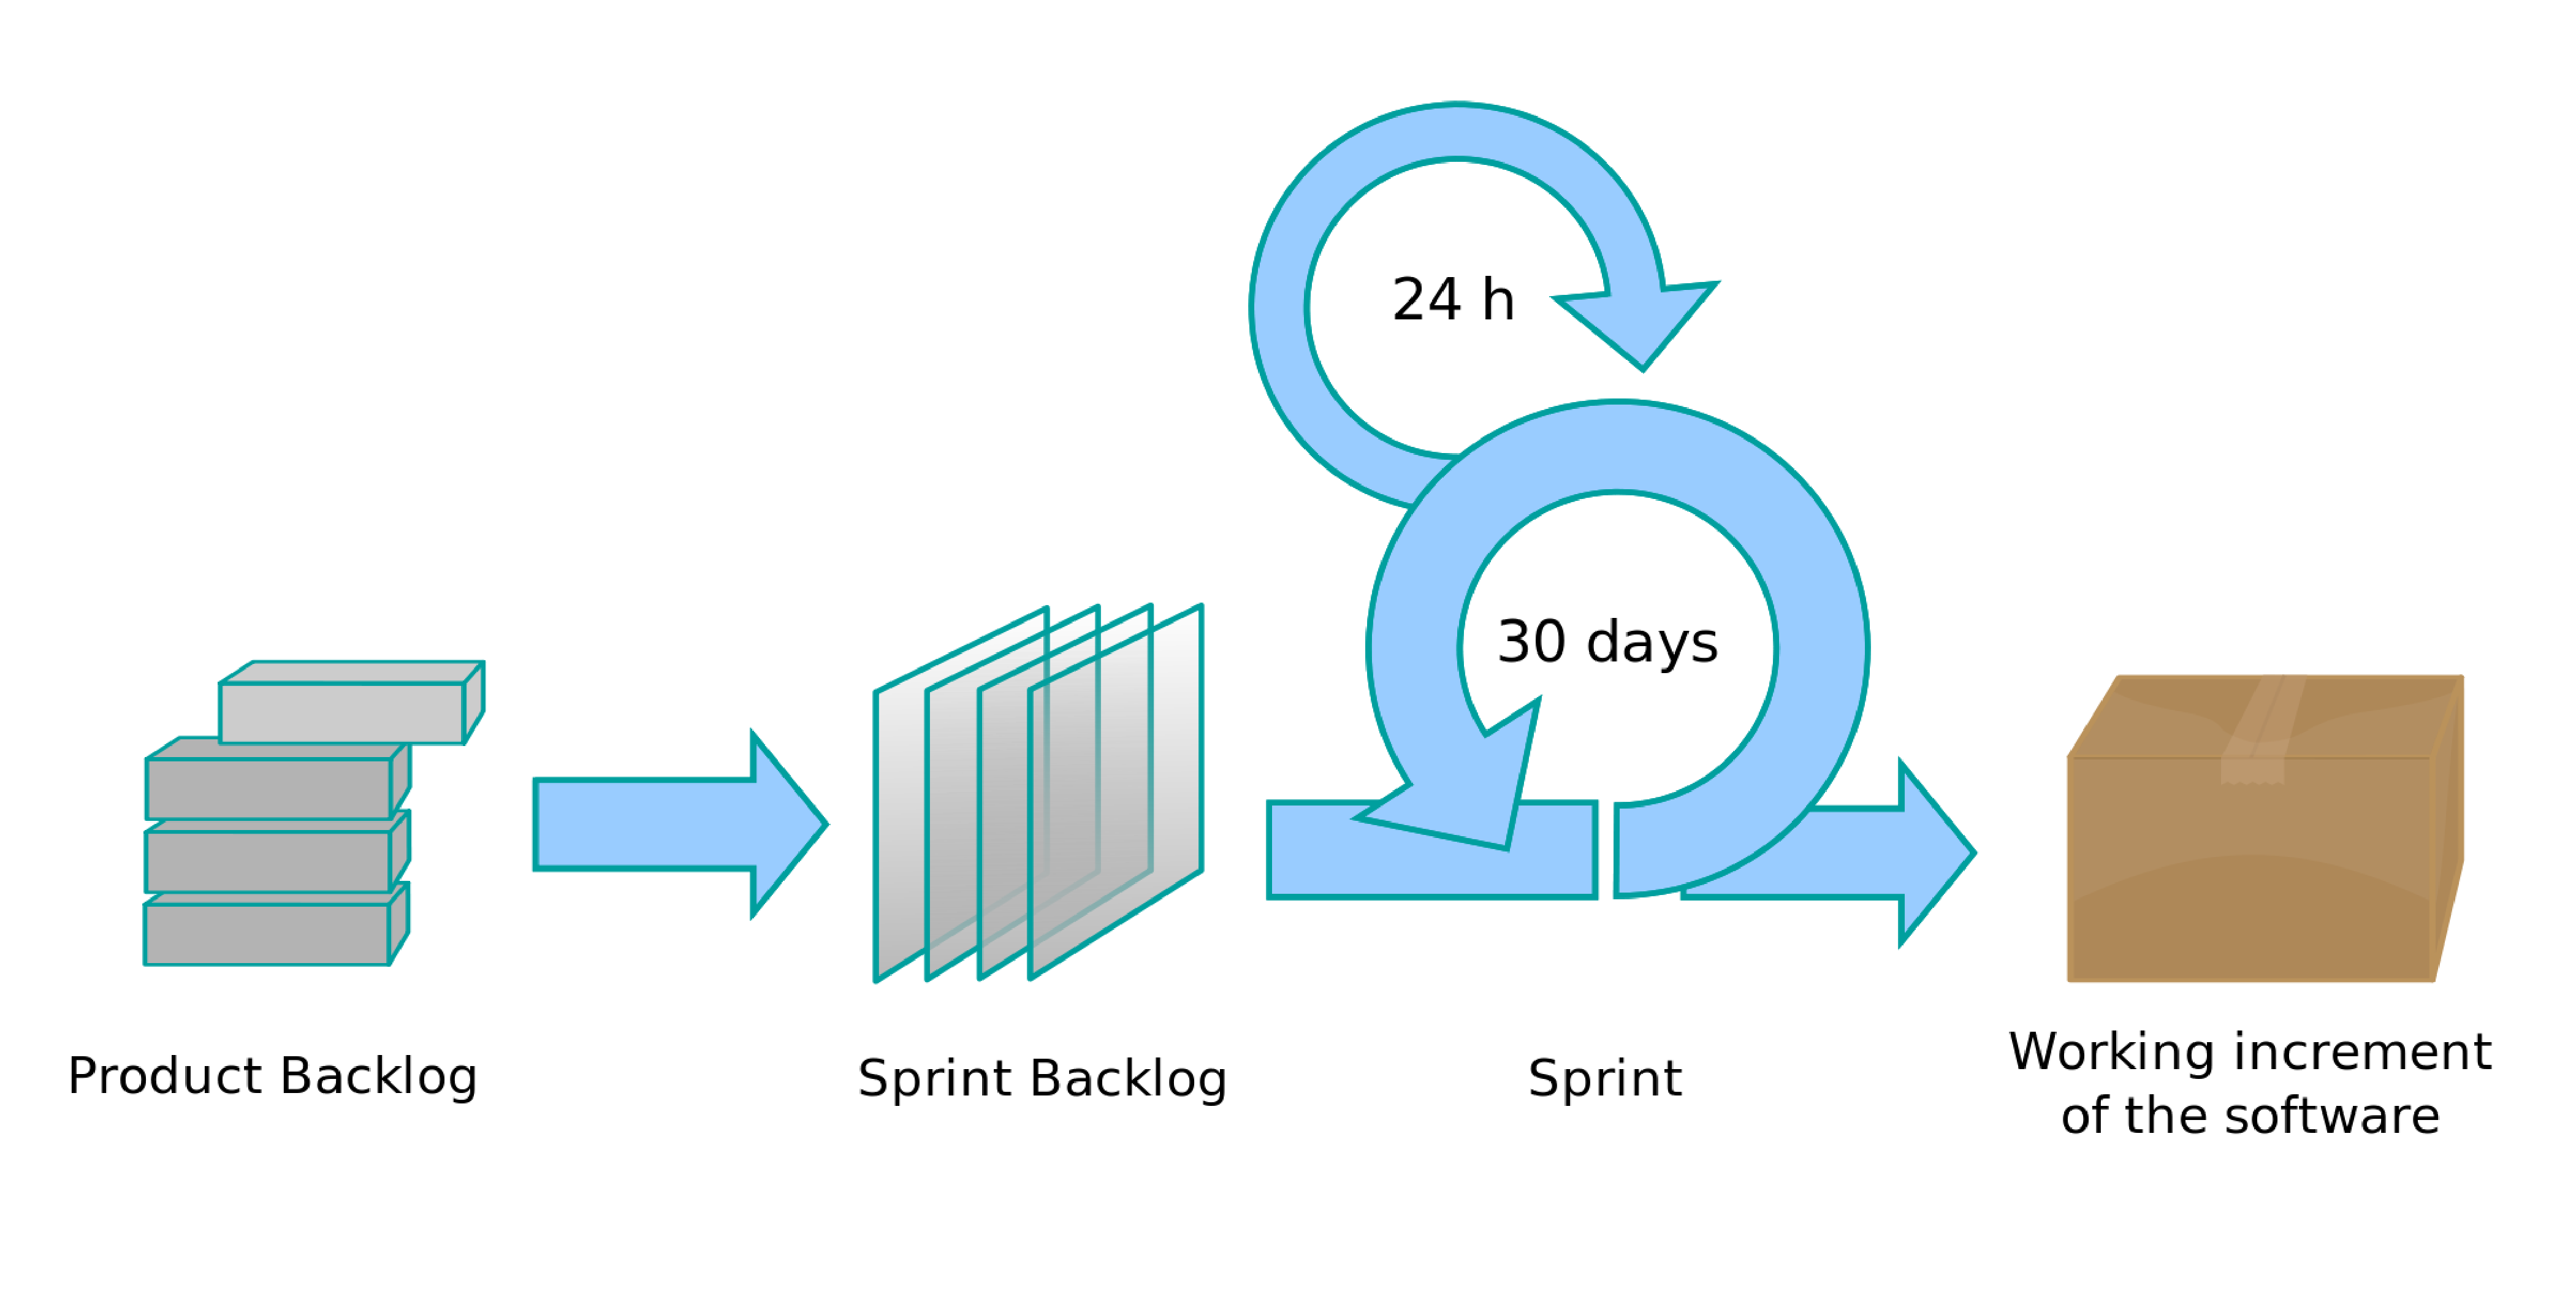
\includegraphics[width=0.95\textwidth]{scrum}
\caption{Scrum \cite{scrumkuva}}
\end{figure}

Kolmas Scrumin perusperiaate, eli sopeutuminen, tulee myös esille monissa eri yhteyksissä ja toimintatavoissa. Edellämainituissa daily-palavereissa yksi tärkeä asia on se, että kaikki projektitiimin jäsenet pääsevät kertomaan mahdollisista ongelmistaan, joita ovat työssään kohdanneet. Tällöin tiimillä on mahdollisuus puuttua näihin ongelmiin heti ja ratkaista ne yhdessä sen sijaan, että tiimin jäsen jäisi yksin ongelmiensa kanssa ja töiden eteneminen mahdollisesti hidastuisi, jolloin myöskään sprintin tavoite ei välttämättä täyttyisi. 

Jokaisen sprintin päätteeksi läpikäytävä retrospektiivi on työn ja työtapojen tarkastelun ohella erittäin hyvä tilaisuus tiimille sopeutumiseen, sillä tilaisuudessa ei ole tarkoitus tuoda esiin vain huonoja toimintatapoja tai ongelmia, vaan ennenkaikkea näihin esille tuleviin kehityskohteisiin yritetään koko tiimin voimin löytää ratkaisuja heti \cite{msretro}. Tällöin ongelmat eivät jää kenenellekään yksin hoidettaviksi, vaan niihin voidaan heti puuttua useamman henkilön voimin. Myös toisessa sprintin päätteeksi läpikäytävässä tapahtumassa, eli sprintin arvioinnissa, on eri sidosryhmillä hyvät mahdollisuudet sopeutumiseen. Tässä tilaisuudessa tilaisuudessa asiakas voi antaa palautetta kehitystiimin suuntaan, kuten myös toisinpäin. Tällöin esimerkiksi kehitystiimi voi ottaa oppia, jos vaikkapa joitain asiakkaan pyyntöjä on ymmärretty väärin ja vastaavasti asiakas voi saada hyvää kokemusta siitä, millä tavalla asiat kannattaa kehitystiimille esittää.

Ylipäänsä Scrumin sprinttiajattelu tarjoaa jatkuvaan sopeutumiseen erittäin hyvät mahdollisuudet. Kun käytännön työssä työn alle otettavat tehtävät lukitaan vain yhdeksi sprintiksi kerrallaan, tiimin on helppo sopeutua muuttuviin vaatimuksiin ja asiakkaan toiveisiin. Esimerkiksi asiakkaalle tärkeä uusi ominaisuus voidaan ottaa heti seuraavassa alkavassa sprintissä työn alle, jos sen prioriteetti on niin tärkeä, että se menee muiden tuotteen backlogin tehtävien edelle. Muutenkin sprintit tarjoavat tiimille mahdollisuuden muuttua tarpeen mukaan nopeasti. Tiimin kokoa voidaan helposti tarpeen mukaan muokata, uusia toimintatapoja käydä retrospektiiveissä läpi sekä suuriakin suunnanmuutoksia projektissa voidaan tehdä helposti verrattuna esimerkiksi vanhaan vesiputousmalliin.

Edellämainittujen tilaisuuksien ohella Scrum-tiimissä on määritelty henkilö, joka mahdollistaa tiimin sopeutumista. Tälle henkilöllä on Scrum-tiimissä oma erityinen roolinsa, aivan kuten tuoteomistajalla ja kehitystiimin jäsenellä. Tätä kutsutaan scrummasteriksi, jonka tehtävänä on toimia palvelevana johtajana. Käytännön tasolla tämä tarkoittaa sitä, yksi kehitystiimin jäsenistä toimii mahdollisten omien tehtäviensä ohella scrummasterin roolissa tai mahdollisesti hänellä ei ole mitään muita tehtäviä kuin scrummasterin tehtävät. Scrummasterin tehtävänä on toimia kehitystiimille mahdollistajana, eli hän ratkaisee kehitystiimin puolesta sellaisia ongelmia, joita esimerkiksi daily-palavereissa tulee esille, jotka haittaavat heidän työntekoaan. Scrummasterin tehtävänä on myös valvoa, että Scrumin käytänteitä toteutetaan ja niistä pidetään kiinni. Tämä tarkoittaa sitä, että scrummaster toimii fasilitaattorina, eli pitää huolen siitä, että esimerkiksi daily-palaverit pidetään, sprintien suunnittelut pidetään ja kaikista määrätyistä aikamääreistä pidetään kiinni. Scrummasterin tehtävänä on huolehtia näille tapahtumille paikat, joissa ne voidaan järjestää. Hän myös toimii yhteydenpitäjänä kehitystiimin ja muiden sidosryhmien välillä siten, että itse kehitystiimin jäsenten työ ei häiriinny turhaan. Täten scrummaster voi esimerkiksi selittää Scrumin periaatteita muille sidosryhmille, jotta päästäisiin mahdollisimman hyvään ymmärrykseen siitä, miksi asioita tulee tehdä Scrumin toimintaperiaatteiden mukaan, jolloin kehitystiimin ei tarvitse huolehtia tämänkaltaisten asioiden selittämisestä muille tahoille.

\section{Laatu}

Tietokoneohjelmistojen laadun merkitys on jatkuvasti yhä suuremmassa roolissa, kun monet yhteiskunnan tärkeistä toiminnoista digitalisoituvat. Tämä tarkoittaa myös sitä, että yhä suuremmassa määrin yhteiskunnan toiminnan kannalta kriittiset palvelut nojaavat ohjelmistojen toimintavarmuuteen. Tämä sama ilmiö on tapahtunut myös teollisuudessa, eikä nykypäivänä oikeastaan ole mitään alaa, jossa tietotekniikka ei tarvittaisi. Laadunvarmistus ja suhtautuminen laadun käsitteeseen poikkeaa hyvin paljon vaiheellisissa ohjelmistotuotantoprosesseissa verrattuna iteratiivisesti toimiviin prosesseihin. Seuraavassa käsitelläänkin näiden erityispiirteitä ja eroavaisuuksia.

\subsection{Laatu vaiheellisissa ohjelmistotuotantoprosesseissa}

Vaiheellisissa ohjelmistotuotantoprosesseissa, kuten esimerkiksi vesiputousmallissa, testaus ja laadunvarmistus on erotettu omaksi erilliseksi vaiheekseen, joka tapahtuu vasta toteutusvaiheen jälkeen \cite{managing}. Tällöin tilanne on se, että koko projekti on toteutettu valmiiksi asti kiinteillä muuttumattomilla vaatimuksilla, jotka on lukittu ennen toteutustyön aloittamista. Testausvaiheessa toteutettua ohjelmisto testataan näitä vaatimuksia vasten, eli pidetään huolta, että nämä vaatimukset täyttyvät. 

Monesti ongelmallista onkin, että asiakas saa toimivan tuotteen vasta tämän testausvaiheen jälkeen ensimmäistä kertaa itselleen testattavaksi, jolloin kyseessä on mahdollisesti alkuperäisten vaatimusten mukaisesti toimiva tuote, mutta käytännössä asiakkaan näkemys ja tarve on voinut muuttua jo monilta osin sinä aikana, kun ohjelmisto on toteutettu. Näin ollen valmiin tuotteen laatu voikin olla asiakkaan mielestä huonompi kuin projektin toteuttajien näkemys on. Kuitenkin teknisellä tasolla vaiheellisissa prosesseissa voidaan panostaa laatuun aivan samalla tapaa kuin iteratiivisissakin prosesseissa. Implementaatiota tehdessä yksikkötestauksen merkitys laadunvarmistuksessa on aivan yhtä suuri kuin iteratiivisissakin prosesseissa.

Kaikenkaikkiaan vaiheellisissa ohjelmistotuotantoprosesseissa testaukseen ja laadunvarmistukseen on hyvät ja kehittyneet keinot, sillä tämä osa-alue on aina ollut mukana omana vaiheenaan prosesseissa \cite{agilequality}. Ongelmaksi näissä prosesseissa laadun kohdalla muodostuukin lähinnä eri osapuolten käsitys laadusta ja mahdolliset asiakkaan muuttuneet tarpeet.

\subsection{Laatu iteratiivisissa ohjelmistotuotantoprosesseissa}

Iteratiivisista ohjelmistotuotantoprosesseista tässä keskitytään erityisesti Scrumiin ja sen suhtautumiseen laatuun. Iteratiivisissa prosesseissa jokaisen sprintin voidaan ajatella toimivan ikäänkuin samalla tavoin kuin kokonaisen vesiputousmallin projektin kaikki vaiheet, sprintin sisältä ei kuitenkaan välttämättä voida selvästi näitä vaiheita erottaa \cite{agilequality}. Kuitenkin toteutustyössä tärkeitä laadunvarmistuksen välineitä ovat esimerkiksi yksikkötestit, joita käytetään aivan samalla tavoin kuin vaiheellisissa prosesseissa. Erona vaiheellisiin prosesseihin, iteratiivisissa prosesseissa testaus tehdään pohjautuen sprintiin valittuihin tehtäviin, joka tarkoittaa sitä, että sprintiin valituille töille on määritetty hyväksymiskriteerit, joissa määritellään milloin haluttu ominaisuus on valmis. Sprintin aikana valmistuvia tehtäviä testataan sitten asetettuja hyväksymiskriteerejä vasten, jotka määritellään yhdessä asiakkaan kanssa.

Sprinteissä tapahtuvan testauksen ja laadunvarmistuksen ohella Software Quality and Methods -julkaisu \cite{agilequality} listaa muutamia muita iteratiivisissa ohjelmistotuotantoprosesseissa yleisesti käytössä olevia toimintatapoja, joiden voidaan katsoa parantavan ohjelmiston laatua:
\begin{itemize}
\item Jatkuvalla integraatiolla tarkoitetaan käytäntöä, jossa ohjelmistoon tehtyjä muutoksia integroidaan jatkuvasti ja muutosten myötä automaattisesti testataan ohjelmiston toiminta ja integraatiot \cite{ci}. Tällaisella käytännöllä kehitystiimillä on jatkuvasti toimiva ohjelmisto, ja kehitystiimi pääsee eroon suuresta riskistä, joka syntyy, kun suuri määrä muutoksia ohjelmistoon otetaan käyttöön samaan aikaan. Kun tehdyt muutokset integroidaan heti valmistumisen jälkeen muuhun järjestelmään, voidaan mahdollisiin virheisiin tai suurempiin ongelmiin puuttua heti. 
\item Jatkuvan integraation palvelimet, kuten esimerkiksi yksi suosituimmista avoimeen lähdekoodiin perustuviasta ratkaisuista, Jenkins \cite{jenkins}, toimivat jatkuvan integraation mahdollistajina. Käytännössä nämä palvelimet aina versiohallinnassa tapahtuvien muutosten yhteydessä buildaavat sovelluksen automaattisesti, ajavat sille kirjoitetut testit ja ottavat sen mahdollisesti käyttöön sovelluspalvelimella. Jatkuvan integraation palvelimet antavat siten heti viestin, mikäli ohjelmiston buildaaminen ei onnistu tai testeissä on virheitä, jolloin kehittäjät tietävät virheistä lähes heti commitin jälkeen \cite{ci}.
\item Usein iteratiivisissa prosesseissa, kuten Scrumissa, on kommunikaatiolla ja yhdessä asiakkaan kanssa työskentelyllä tärkeä rooli, jonka voidaan nähdä parantavan ohjelmiston laatua. Tällä tavoin asiakkaaseen saadaan helposti yhteyttä ja hänen kanssaan voidaan jatkuvasti kommunikoida, mikä edistää esimerkiksi epäselvien vaatimusten selvityksessä ja niiden jatkuvaa parantamista \cite{agilequality}. Myös esimerkiksi Scrum-tiimin tuoteomistaja on usein asiakkaan edustaja, jolloin asiakkaalla on jatkuvasti todella hyvä näkyvyys siihen, mitä ollaan tekemässä, kun tuoteomistaja vastaa tuotebacklogin priorisoinnista. Tällöin asiakas voi varmistaa sen, että kehitystiimi työskentelee jatkuvasti sellaisten töiden parissa, jotka ovat asiakkaalle kaikkein hyödyllisimpiä. Tilanne, jossa tuoteomistaja on nimetty asiakkaan puolesta, on kommunikaatiomahdollisuuksiensa puolesta lähes ihanteellinen, sillä Scrumissa tuoteomistaja on henkilö, jolla tulisi olla jatkuvasti kaikkein paras visio siitä, mitä ollaan tekemässä ja mitä ohjelmistoon seuraavaksi halutaan tehdä \cite{scrumguide}.
\end{itemize}

Ketterissä menetelmissä kehittäjillä on enemmän vastuuta ohjelmiston laadusta kuin perinteisissa vaiheellisissa ohjelmistotuotantoprosesseissa. Tämä ei tule varsinaisesti esille suoraan iteratiivisissa ohjelmistotuotantoprosesseissa, mutta tämä johtuu hyvin pitkälti siitä, että näissä prosesseissa pelkän suunnittelun määrä on usein minimoitu ja jonkinlaista toteutusta lähdetään tekemään lähes heti. Tällöin laadunvarmistusta joudutaan tekemään paljon jo kehittäjien toimesta ohjelmistoa implementoidessa \cite{agilequality}. Nopeisiin sykleihin, jatkuvaan integraatioon ja tuotteen toimituksiin on ohjelmistoalalla iteratiivisissa prosesseissa sopeuduttu ohjelmistokehityksen toimintatapoja on muokkaamalla siten, että ohjelmoinnissa käytetään menetelmiä, joiden voidaan katsoa edistävän laadunvarmistusta. Yksi tärkeistä laatua edistävistä ohjelmistokehityksen malleista on TDD, jota käsitellään seuraavassa.

\section{TDD}

TDD, eli Test-driven development, tarkoittaa testivetoista ohjelmistokehitystä. TDD poikkeaa edellä esitetyistä malleista siinä, että siinä missä edellä esitellyt mallit kattavat koko ohjelmistokehitysprosessin, ottaa TDD kantaa ainoastaan edeltävissä malleissa esiintyneisiin käytännön toteutus- ja testausvaiheisiin. Käytännössä siis nykyään ohjelmistoprojekteissa valitaan jokin koko ohjelmistokehitysprosessin kattava malli, kuten Scrum, jossa sitten hyödynnetään TDD:tä ja sen ohjelmointikäytänteitä. Seuraavassa esitelläänkin TDD:n keskeisimmät ideat ja toimintaperiaatteet, joita käytännön ohjelmistokehityksessä usein noudatetaan.

Yksinkertaistettuna testivetoisessa ohjelmistokehityksessa ideana on se, että testit kirjoitetaan ennen kuin kirjoitetaan riviäkään koodia. Käytännössä tämä tarkoittaa sitä, että ennen ohjelmointia testeillä määritellään se, mitä seuraavaksi kirjoitettavan metodin olisi tarkoitus tehdä. Työvaiheet tässä prosessissa ovat seuraavanlaiset \cite{tdd}:
\begin{itemize}
\item Kirjoitetaan testi, joka ei mene läpi.
\item Kirjoitetaan koodi, joka läpäisee testin. Tässä vaiheessa ei ole vaatimuksia koodin optimoinnille tai laadulle.
\item Ajetaan testit ja todetaan niiden menevän läpi.
\item Refaktorointi. Refaktoroidaan kohdassa kaksi kirjoitettua koodia, eli esimerkiksi poistetaan siitä kaikenlaiset epäloogisuudet, siirretään metodi loogisesti oikeaan paikkaan ja nimetään se järkevästi.
\item Aloitetaan prosessi alusta.
\end{itemize}

TDD:n voidaan katsoa edistävän työskentelyä ainakin neljästä eri näkökulmasta \cite{tddeff}. Ensiksikin kehittäjä saa jatkuvaa palautetta työstään viiveettä. Hän näkee heti toimiiko tekemänsä koodi oikein ja rikkooko se mahdollisesti muita toiminnallisuuksia ja niiden testejä. Tällöin kehittäjä pystyy heti korjaamaan virheensä, eikä niitä ehdi kasaantua kerralla paljoa.

Samalla tämä yhteen metodiin keskittyminen kerrallaan ohjaa ja jaksottaa kehittäjän työskentelyä. Tämä tarkoittaa sitä, että kehittäjä keskittyy yhteen tehtävään kerrallaan, kunnes saa valmiiksi toimivan testatun kokonaisuuden. Tämän myötä kehittäjien on välttämätöntä myös pilkkoa työtään pienempiin osiin siten, että tällainen tehtävä kerrallaan läpiviety kehitys on edes mahdollista \cite{tddeff}. Kun tehtävät pilkotaan riittävän pieniksi, kehittäjien on helpompi arvioida niihin kuluvaa aikaa, heillä on parempi käsitys siitä, mitä jonkin asian valmistuminen vielä vaatii ja he kykenevät hallitsemaan omia työn alla olevia töitään helpommin.

Kolmantena TDD tarjoaa omalta osaltaan yhden keinon laadunvarmistukseen. Kun ohjelmistoa kehitetään TDD:n keinoin, on jatkuvasti olemassa setti testejä, jotka parhaassa tapauksessa kattavat koko ohjelmiston, jos se on alusta alkaen kehitetty TDD:llä \cite{tddeff}. Sen lisäksi, että TDD:n myötä syntyvä testisetti on kattava, sitä myös ajetaan usein, sillä kaikkien uusien ominaisuuksien yhteydessä tulisi tarkistaa aina kaikkien testien toimivuus, jotta vältytään mahdollisilta uusien ominaisuuksien luomilta sivuvaikutuksilta.
 
Viimeiseksi TDD:ssä keskitytään ennen kaikkea matalalla tasolla koodin testaamiseen. Kun liikutaan yksittäisten metodien tasolla, on ohjelmoijalla usein hyvä näkemys siitä, mitä kirjoitettavan metodin olisi tarkoitus tehdä. Tällöin koodin laatu paranee ainakin tällä matalalla tasolla, mutta TDD ei ota kantaa, eikä auta ohjelmoijaa ymmärtämään korkeamman tason toiminnallisia vaatimuksia tai suurempia kokonaisuuksia \cite{tdd}. Tähän ongelmaan ratkaisuksi on lähivuosina kehitetty toimintatapoja, joilla pystytään hallitsemaan paremmin edellämainittujen korkeamman tason vaatimusten täyttymistä. Näitä menetelmiä ovat muun muassa Acceptance Test-Driven Development (ATDD) sekä Behaviour-Driven Development (BDD), joita käsitellään tarkemmin jäljempänä.

Vuonna 2005 julkaistussa tutkimuksessa \cite{tddeff} suurimpana kysymyksenä oli selvittää TDD:n vaikutusta tuottavuuteen. Tutkimuksessa todettiin testilähtöisen kehityksen todella lisäävän kehittäjien tuottavuutta. Tähän löydettiin tutkimuksessa \cite{tddeff} useita syitä. Yksi näistä oli jo edelläkin mainittu tehtävien pilkkominen ja sen myötä niihin keskittyminen. Näillä toimenpiteillä tehtävät ovat helpommin ymmärrettäviä kokonaisuuksia, jotka voidaan helposti toteuttaa kerralla. Tutkimus myös toteaa \cite{tddeff}, että testivetoisessa kehityksessä huonot ja tehottomat toimintatavat hylätään verrattain nopeasti ja ne korvataan paremmilla. Useimmissa prosessimalleissa tällaiset päätökset tekevät kehittäjät itse, eli näitä parannuksia ei osoiteta mistään ylemmältä taholta. Esimerkiksi Scrumissa kehitystiimi itse käy jokaisen sprintin jälkeen retrospektiivissa läpi omaa toimintaansa ja yrittää löytää siitä kehityskohteita \cite{scrumguide}. Tämä jatkuva toimintatapojen tehostaminen johtaa myös nopeaan oppimiseen. TDD laskee myös kynnystä asioiden uudelleen tekemiselle ja refaktoroinnille \cite{tddeff}. Kun ohjelmisto on toteutettu pienistä erikseen testatuista osista, on helppoa lähteä korjaamaan yhtä hajonnutta testiä, sillä hajoamisen syy on usein helppo löytää, kun testi kattaa vain yhden pienen osan ohjelmistosta, esimerkiksi yhden metodin, jonka tehtävän pitäisi olla helposti selitettävä.

Kaikenkaikkiaan vuoden 2005 tutkimuksessa \cite{tddeff} päädyttiin tulokseen, jonka mukaan testivetoinen kehitys todellakin parantaa työn tuottavuutta edellämainittujen seikkojen myötä. Samalla tutkimuksessa kuitenkin todetaan, että testivetoinen ohjelmistokehitys ei suoranaisesti paranna ohjelmistojen laatua. Tämä johtui siitä, että vaikka ohjelmistokehittäjät kirjoivat TDD:tä käyttäessään määrällisesti enemmän testejä, testien laatu riippui hyvin paljon kehittäjän kokemuksesta tehdä töitä testivetoisesti \cite{tddeff}. Testivetoisessa kehityksessä testeillä osaltaan ohjataan kehittäjän työtä, eli kehittäjä kertoo testeillä itselleen mitä hänen pitäisi seuraavaksi tehdä. Taito kirjoittaa hyviä testejä, jotka testaavat oikeita asioita syntyy vain testejä kirjoittamalla, eli tässä tilanteessa kokemus ja työskentelytapaan tottuminen tuovat lisää tehokkuutta työskentelyyn. Toisaalta myös matalan tason yksikkötesteistä saatavan hyödyn voitiin katsoa häviävän siinä, että kehittäjät pystyivät monissa tilanteissa ohjelmaa tarkastelemalla helposti toteamaan saman asian kuin mitä yksikkötesti testaa \cite{tddeff}.

\begin{figure}
\centering
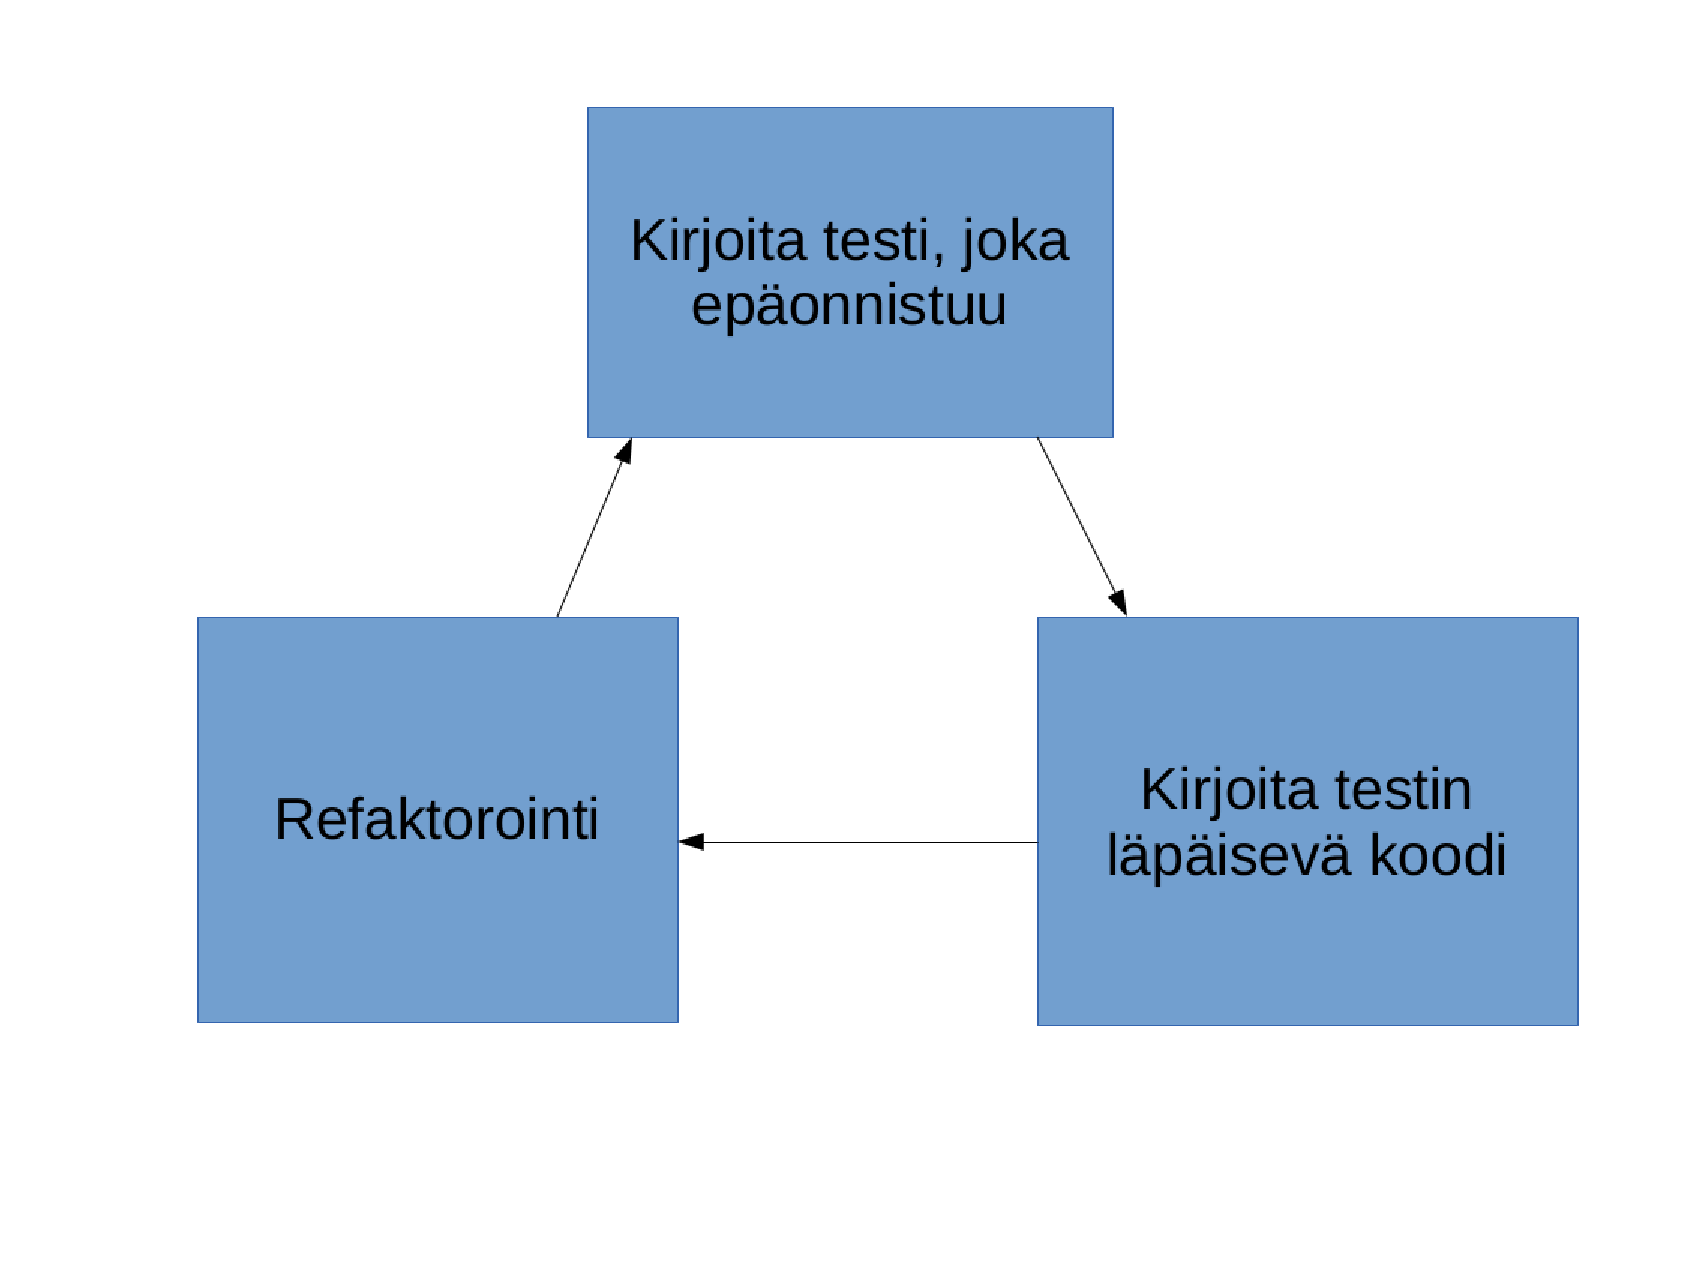
\includegraphics[width=0.95\textwidth]{tdd.eps}
\caption{TDD-työvaiheet}
\end{figure}

\section{ATDD}
ATDD eli Acceptance Test-driven development tarkoittaa nimensä mukaisesti hyväksymistestilähtöistä ohjelmistokehitystä. ATDD:ssä kehittäjät, käyttäjät ja testaajat yhdessä määrittelevät ohjelmistolle hyväksymiskriteerit, joiden pohjalta ohjelmistoa lähdetään kehittämään \cite{difference}.  

ATDD:llä ja BDD:llä tarkoitetaan useissa yhteyksissä samaa asiaa, sillä termit ovat alalla vielä niin uusia, eikä vakiintuneita käytäntöjä ole. Tämän myötä termistö ja nimet muuttuvat jatkuvasti kehityksen myötä. Hyvin pitkälti ATDD:n ja BDD:n ero voidaan nähdä löytyvän ennemminkin siinä, minkä tasoiseen testaamiseen niissä keskitytään \cite{difference}. Toinen tasoista on ATDD:n hyväksymistestilähtöinen malli, jossa keskitytään automaattisiin hyväksymistesteihin, joilla määritellään selviä vaatimuksia kehittäjätiimille, jotka toteutetun järjestelmän tulee täyttää \cite{specification}.

BDD sen sijaan toimii tasolla, jossa määritellään erilaisia skenaarioita, joiden tavalla järjestelmän tulisi toimia. BDD:n mallissa keskeistä on ennenkaikkea luoda ymmärrystä kehittäjien ja muiden sidosryhmien, kuten esimerkiksi asiakkaan edustajien, välille \cite{specification}. Tämän ohella kuitenkin BDD auttaa myös välttämään toiminnallisia regressiobugeja aivan kuten ATDD:kin. Kummatkin tasoista toteuttavat kuitenkin myös osaltaan esimerkein määrittelyn periaatteita ja estävät toiminnallisia regressiobugeja syntymästä. ATDD:n tason voidaan nähdä myös soveltuvan paremmin tietynlaisiin toimintaympäristöihin, kun taas BDD:n taso toimii toisaalla paremmin. Gojko Adzic kirjoittaa Specification by Example -kirjassaan \cite{specification} ATDD:n mallin olevan hyödyllisempi, jos ollaan toteuttamassa ohjelmistoa, jossa on useita laatuun liittyviä haasteita. BDD:n tason taas voidaan nähdä sopivan paremmin tilanteeseen, jossa ei ole suurempia ongelmia ja BDD:tä voidaankin käyttää lähinnä selittämään asioita. 

Kumpikin malli kuitenkin tuottaa erittäin hyvää dokumentaatiota järjestelmästä ilman erillistä panostusta sen tekemiseen, ja tämän voidaankin nähdä olevan yksi suurimmista eduista, joita saavutetaan käyttämällä ATDD:tä tai BDD:tä \cite{specification}. Haastatteluissaan Adzic sai kirjassaan selville jopa sen, että hyvin tehtynä selkeät, ylläpidettävät testit monesti jopa riittivät ainoaksi dokumentaatioksi järjestelmästä, sillä niiden käyttö oli helpompaa kuin erillisten dokumenttien tuottaminen \cite{specification}. Useat BDD- ja ATDD-työkalut, kuten esimerkiksi Cucumber \cite{cucumber} myös tukevat automaattisesti esimerkiksi nettisivujen luontia testeistä, jolloin niistä saadaan dokumentaation kaltainen artefakti hyvin pienellä vaivalla.

\chapter{Behaviour-driven development}

\section{BDD:n lähtökohdat ohjelmistokehitystä tukevana menetelmänä}
BDD, eli Behaviour-driven development, on nimensä mukaisesti ohjelmistokehityksen malli, jossa ohjelmistojen kehityksen lähtökohtana on niiden käyttäytyminen \cite{bddintro}. Toisin kuin edellä käsitellyssä ATDD:ssä, voidaan BDD:n painottavan enemmän kommunikaation merkitystä sidosryhmien välillä kuin vain automaattisten hyväksymistestien luontia. Yksi keinoista, joilla monissa BDD-testikehyksissä parannetaan kommunikaatiota ja yhteisymmärrystä eri sidosryhmien, kuten ohjelmistokehittäjien ja toimialan asiantuntijoiden välillä, on lähellä luonnollista kieltä oleva kieli, jolla testejä määritellään \cite{cucumberbook}. Esimerkiksi seuraavanlaisella muotoilulla voidaan määritellä testiskenaario Cucumber-testikehyksessä \cite{cucumber}:

\begin{verbatim}
Feature: Generation
  In order to finish the thesis
  As a student
  I want to generate good BDD-examples

  Scenario: Generate example of behaviour
    Given I have program running
    When I press generate
    Then the result should be an example behaviour on the screen
\end{verbatim} 

Kuten skenaarion muotoilusta voidaan nähdä, BDD:ssä testataan ennen kaikkea sitä, toimiiko ohjelmisto oikein ja halutulla tavalla, eli sen käyttäytymistä. Verrattuna TDD:n matalan tason testeihin, joissa keskitytään yhden metodin toimintaan kerrallaan, ero on merkittävä. Yksi merkittävistä asioista, joiden avulla BDD:llä voidaan ohjata ohjelmistokehitysprosessia on tapa, jossa toimintojen tuottama lisäarvo otetaan huomioon. Tällöin eniten lisäarvoa tuottavia ominaisuuksia voidaan ensimmäisenä lähtea kehittämään ja niille voidaan luoda BDD-testit, jotka nimetään sen mukaan, mitä järjestelmän halutaan tekevän \cite{bddintro}.

Monilta osin BDD perustuu Test-driven developmentin parhaisiin käytänteisiin ja samalla BDD:n tarkoituksena on formalisoida niitä \cite{cucumberbook}. TDD:n voidaankin ajatella auttavan kehittäjiä toteuttamaan ratkaisun oikein, kun taas ATDD ja BDD auttavat kehittäjiä toteuttamaan oikean ratkaisun \cite{cucumberbook}. Sekä TDD:stä, että BDD:stä kummastakin löytyy komponentit, joilla on helppo selventää eroja näiden kahden menetelmän välillä. Siinä missä TDD:ssä keskitytään testeihin, joilla testataan yhtä luokkaa ja sen metodien toimintaa, BDD:ssä vastaava komponentti on esimerkki, jolla kuvaillaan yhden luokan toivottua käyttäytymistä \cite{tddbdd}. Siinä missä TDD:ssä testien odotetaan menevän läpi, BDD:ssä halutaan ohjelmiston käyttäytyvän oikein. BDD:ssä testeillä varmistetaan, että toiminnallisuus on oikea, eli tuottaa mahdollisimman paljon arvoa asiakkaalle, kun TDD:ssä testit testaavat toiminnallisuutta vain matalalla tasolla \cite{tddbdd}, eivätkä ne ota asiakkaan tarpeita niinkään huomioon.

\section{Teknologioista}
\subsection{Yleistä teknologioista}
Behaviour-driven developmentia varten on olemassa useita eri testikehyksiä, jotka soveltuvat eri tarkoituksiin. Eräitä esimerkkejä näistä ovat Cucumber \cite{cucumber}, Jasmine \cite{jasmine}, Specflow \cite{specflow} ja RSpec \cite{rspec}. Mainittujen testikehysten suurin ero on alustat, joita ne tukevat. Jasmine on JavaScript-ohjelmointikielelle tehty testikehys, kun taas SpecFlow on ratkaisu Microsoftin .NET-alustan BDD-testaamiseen. Cucumber ja RSpec pohjautuvat molemmat Ruby-ohjelmointikieleen, mutta ne poikkeavat toisistaan kuitenkin muuten varsin paljon. Siinä missä RSpec on ainoastaan Rubya tukeva kehys, jolla voidaan toteuttaa niin TDD- kuin BDD-testaustakin, niin Cucumber kehyksenä korostaa erityisesti määrittelyjen luettavuutta ja ymmärrettävyyttä. RSpec ei tarjoa mahdollisuutta määritellä erikseen lähellä selkokieltä olevia kuvauksia käyttäytymisestä, kuten Cucumberissa, vaan siinä koko testi on yhdessä yksittäisessä tiedostossa. Tällöin luettavuusero on varsin merkittävä, kun otetaan huomioon BDD:n lähtökohta kommunikaation parantajana:

RSpec:
\begin{verbatim}
# example_spec.rb

require 'spec_helper'
describe "exampletest" do
  it "should have a page titled Example at '/example'" do
   get '/example'
   response.should have_xpath("//title", :text => "Example")
 end
end
\end{verbatim} 

Vastaavasti Cucumberissä on erillisessä feature-tiedostossa määritelty luonnollisen kaltaisella kielellä eri skenaariot, joiden mukaan ohjelman halutaan toimivan. Tämän lisäksi on sitten erillinen Rubylla kirjoitettu tiedosto, jossa määritellään, mitä feature-tiedostossa käytetyt stepit tekevät. Tässä siis selvästi erotellaan liiketoiminnan kannalta tärkeät määrittelyt erikseen lähes selkokieliseen muotoon, jolloin niiden tulkinta on verrattain helpompaa kuin esimerkiksi RSpecin tapauksessa suoraan Ruby-koodin lukeminen. Edellä esitellyn RSpec-testin kaltainen testi Cucumberilla voitaisiin toteuttaa esimerkiksi seuraavalla tavalla:

Cucumber:
\begin{verbatim}
# example.feature

Scenario: As a user I want to see correct page title
  Given I am on the home page
  When I go to example page
  Then I should be on the page with the title: "Example" 

# example_steps.rb

Given /^I am on the home page$/ do
  visit '/'
end

When /^I go to the example page$/ do
  visit '/example'
end

Then /^I should be on the page with the title: "([^"]*)"$/
do |page_title|
  response.should have_xpath("//title", :text => "#{page_title}")
end
\end{verbatim}

Esimerkeistä voidaan huomata, kuinka Cucumberilla esimerkkiskenaariosta tulee paljon helpommin luettava henkilöille, jotka eivät ole teknisesti orientoituneita. Siinä missä RSpec-testissä samaan tiedostoon on määritetty testin kuvaus kuin sen toiminnalisuuskin, niin Cucumberissa testi on selvästi erikseen kuvattu feature-tiedostossa, jolloin eri sidosryhmien edustajat voivat keskittyä vain sen sisältöön, eikä tekninen aineisto, eli eri steppien määritykset, ole sekoittamassa asiaan perehtymätöntä henkilöä.

Yhteistä lähes kaikille BDD-testikehyksille on niiden käyttämä testitapausten muoto yleisellä tasolla. Dan North esittelee tämän muodon Behaviour-driven developmentin konseptia esittelevässä blogitekstissään \cite{bddintro}. Perinteinen pohja käyttäjätarinoille koostuu usein jotakuinkin seuraavanlaisista osista:
\begin{itemize}
\item Roolissa A
\item Haluan tehdä asian B
\item Jotta tapahtuu asia C
\end{itemize}
Tämä kyseisenlainen pohja toimii myös Northin määrittelemän testitapausten muodon pohjana. Tästä mallista North kehitti uuden mallin, jonka avulla voidaan käyttäjätarinat kirjoittaa suoraan hyväksyntätestien muotoon.
\begin{itemize}
\item Given (what is known/done beforehand)
\item When (something is done)
\item Then (something happens)
\end{itemize}
Tällaista Given-When-Then -muotoa käyttävää suuri osa BDD-testikehyksistä testiensä määrittämiseen. Poikkeuksiakin toki on, esimerkiksi aiemmin esimerkkinä ollut RSpec-testikehys Rubylle \cite{rspec}, jossa ei ole erikseen määrittelyjä testitapauksille, vaan kaikki sisältö löytyy koodin seasta. Esimerkiksi seuraavasta RSpec-testistä voidaan löytää vastaavat osat:
\begin{verbatim}
require 'spec_helper'

describe Example do
  it "is not valid without a title" do
    example = Example.new(title: nil)
    example.should_not be_valid
  end
end
\end{verbatim}
Tässä voidaan ajatella, että pohjatietona, eli Given-osiona olisi tilanne, jossa on mahdollista luoda uusi Example. When-kohtana olisi Example.new(title: nil) eli luodaan uusi Example. Tällöin odotetaan tuloksena, että uusi Example ei olisi validi, mikä vastaisi siis Then-kohtaa Dan Northin muodossa. Voidaan kuitenkin miettiä, onko välttämättä hyödyllistä yrittää puristaa jokaista testikehystä ennaltamääritettyyn muotoon, sillä RSpec poikkeaa muista kehyksistä muutenkin verrattain paljon sen tarjotessa mahdollisuudet laajemminkin testivetoiseen kehitykseen Rubylla kuin vain BDD:n toiminnallisuuksia.

Muista testikehyksistä esimerkiksi Cucumber \cite{cucumberbook} käyttää täysin Dan Northin määrittelemää muotoa \cite{bddintro} testeilleen, kun taas JavaScript-testikirjasto Jasminen \cite{jasmine} ratkaisu on hyvin samanlainen kuin RSpecin ratkaisu, eli Jasminessakaan ei ole erikseen määritelty luonnollisella kielellä testejä erikseen. Specflow \cite{specflow}, joka on testikehys .NET, Windows Phone ja Mono-alustoille, on sen sijaan toteutettu vastaamaan Dan Northin määrittelemää mallia, eli Given-When-Then -malliset määritykset testiesimerkeille toteutetaan siinä erikseen ja näille määrityksille ohjelmoidaan tulkit, joilla määritellään mitä testit tekevät.

\subsection{Parsereista}
Yksi tärkeä osa monia BDD-testikehyksiä on niiden käyttämät parserit, joilla tulkitaan määriteltyjä testitapauksia ajettavaksi ohjelmakoodiksi. Näillä parsereilla on kaikilla jokin hyvin määritelty syntaksinsa, jota ne ymmärtävät. Yksi parsereista on esimerkiksi avoimen lähdekoodin Gherkin \cite{gherkin}, jota käyttävät Cucumber \cite{cucumber} ja sen sukuiset BDD-testikehykset, kuten esimerkiksi SpecFlow \cite{specflow}. Gherkinin syntaksi on hyvin yksinkertainen, joka edesauttaa sitä, että eri sidosryhmien edustajat ymmärtävät ja parhaassa tapauksessa voivat jopa itse luoda uusia testitapauksia. Tällöin tarvitaan erityisesti kehitystiimin ja muiden sidosryhmien yhteistyötä, sillä tässäkin tapauksessa kehitystiimin tehtäväksi jää kirjoittaa testitapauksia vastaava ohjelmakoodi, jotta testitapauksista saadaan toimivia. Martin Fowler kirjoittaakin blogissaan \cite{businessdsl}, että ennen kaikkea tärkeää ja hyödyllistä on se, että sidosryhmien edustajat kykenet lukemaan ja ymmärtämään koodia, tai tässä tapauksessa testitapausten kuvauksia, sillä se toimii äärimmäisen hyvänä kommunikaatiovälineenä eri osapuolten välillä. Seuraavassa on esimerkki Gherkin-dokumentista, jossa määritellään esimerkkiskenaario:
\begin{verbatim}
Feature: Software installation
  Scenario: Uninstall software
    Given a software named "example" exists
    When I press uninstall software
    Then the software named "example" should be removed
\end{verbatim}
Tässä esimerkissä ainoat kohdat, jotka määritellään Gherkinin syntaksissa, ovat kaikilla riveillä niiden alut, eli Feature, Scenario, Given, When ja Then \cite{gherkin2}. Kaikki muu sisältö, mitä testitapaukset sisältävät, on testien kirjoittajan itse luomaa sisältöä, eli kaikki muut kohdat tulee määritellä steppien kuvauksissa testikehyksen käyttämällä ohjelmointikielellä. Cucumberin tapauksessa tämä voitaisiin tehdä esimerkiksi Rubylla tai jollakin muulla ohjelmointikielellä, jota Cucumber tukee, kuten esimerkiksi Javalla. Edeltävän esimerkin Given-kohta voitaisiin määritellä toimivaksi testiksi esimerkiksi Java-ohjelmointikieltä käyttäen seuraavalla tavalla:
\begin{verbatim}
@Given("a software named (.*) exists")
public void softwareExists(string software) {
    // Tässä voitaisiin tehdä ohjelmistolla mitä tahansa,
    // esimerkissä halutaan hakea ohjelmistoa
    // sen nimellä SoftwareServiceltä
    getSoftwareService.findSoftware(software);
}
\end{verbatim} 

Gherkinin sijasta monet BDD-testikehykset käyttävät omia parsereitaan. Esimerkiksi RSpec \cite{rspec} ja Jasmine \cite{jasmine} eivät käytä Gherkiniä, vaan niissä on toteutettu omat parserit testien tulkkaamiseen. Yksi eduista, joita saavutetaan yhden parserin yleisyydellä eri testikehyksissä, on se, että tämä edesauttaa testien uudelleenkäytettävyyttä. Kun eri testikehykset käyttävät samaa parseria, niin samat testimääritykset toimivat niille kaikille. Tämä onkin yksi merkittävä havainto etsittäessä ratkaisua tutkielman tutkimuskysymykseen mobiilialustojen BDD-testaamisesta yhdellä testisetillä. Tätä käsitellään myöhemmin lisää kappaleessa \ref{chap:platforms}.

\chapter{BDD:n tarjoamat liiketoiminnalliset edut}
Behaviour-driven developmentin voidaan nähdä tarjoavan muitakin hyötyjä sen lisäksi, että se toimii käytännön tapana kehittää ohjelmistoja teknisellä tasolla ohjelmistokehittäjien toimesta. Yksi tärkeimmistä lähtökohdista, joille BDD:n käytänteet on kehitetty, on kommunikaation lisääminen ja parantaminen asiakkaan ja kehitystiimin välillä \cite{specification}. Välillisesti tämän kommunikaation lisäämisen myötä BDD:n käytöllä pyritään toteuttamaan jatkuvasti entistä paremmin oikeita asioita, eli pyritään minimoimaan eri sidosryhmien välisiä näkemyseroja toiminnallisuuksien välillä. Tähän päästään erityisesti sillä, että asiakkaan kanssa yhdessä määritellään testiesimerkkejä ja toiminnallisuuksia \cite{businessdsl}.  

\section{Asiakkaan käyttäjätarinoista hyväksymistesteiksi}
Kuten edellä mainittiin, on yksi suurimmista BDD:n tarjoamista eduista sen luomat mahdollisuudet työskennellä yhdessä asiakkaan kanssa tuotetun työn arvon maksimoimiseksi. Jos toiminnallisia vaatimuksia määritellään jatkuvasti yhdessä asiakkaan kanssa, ei missään vaiheessa pitäisi syntyä tilannetta, jossa kehitystiimi toteuttaa ominaisuuksia, jotka ovat vääriä tai valmistuessaan jo vanhentuneita tai hyödyttömiä asiakkaan liiketoiminnan kannalta. Erityisen hyvin tällaiseen tilanteeseen päästään, kun BDD:n toimintatavat yhdistetään Scrumiin tai johonkin muuhun inkrementaaliseen prosessimalliin, jossa vaatimuksia ei lyödä heti projektin alussa lukkoon, vaan niitä työstetään jatkuvasti projektin edetessä.

Esimerkiksi Scrumin \cite{scrumguide} yhteydessä BDD:n käytäntöjä voitaisiin hyödyntää seuraavalla tavalla:
\begin{itemize}
\item Product ownerin johdolla tehtävässä tuotebacklogin groomauksessa, eli siistimisessä ja priorisoinnissa voidaan yhdessä asiakkaan kanssa määritellä tuleville toiminnallisuuksille hyväksymiskriteereitä, eli käytännössä kriteereitä sille, milloin voidaan katsoa jonkin ominaisuuden olevan valmis
\item Samalla backlogin groomauksessa voitaisiin vaatimukset kirjoittaa yhdessä asiakkaan kanssa suoraan oikeaan muotoon BDD:tä varten, eli käyttäen esimerkiksi Gherkinin syntaksia, jos projektissa käytetty BDD-testikehys sitä käyttäisi.
\item Mahdollisesti vaatimuksia voitaisiin määritellä myös erillisessä tilaisuudessa, jos sen koettaisiin olevan liian raskasta groomauksen yhteydessä.
\item Sprint planningissa sprintiin mukaan otettavia töitä arvioitaisiin testiesimerkkien muotoon tehtyjen vaatimusmäärittelyjen pohjalta.
\item Sprinttien aikana kehitystiimi toteuttaa ominaisuuksia määriteltyjen testitapausten avulla. Kehitystiimi toteuttaa ensin määritellyille testitapauksille testin teknisen osan, eli toimivan koodin ensin testille, jotta testiä voidaan käyttää ja tämän jälkeen vielä ohjelmakoodi itse ominaisuudelle, jotta testi menee läpi. 
\item Epäselvissä tilanteissa määriteltyjä testejä voidaan käydä läpi yhdessä product ownerin kanssa, jolla pitäisi jatkuvasti olla projektissa paras tieto siitä, mitä halutaan toteuttaa. 
\end{itemize}
Tämä on vain esimerkki siitä, kuinka BDD:n toimintatavat voitaisiin yhdistään käytössä oleviin vakiintuneisiin ohjelmistokehityksen prosessimalleihin. Käytännössä kuitenkin tavat voivat vaihdella tiimistä ja projektista riippuen sen mukaan, mikä parhaiten oikeasti toimii. Mitään tarkasti määriteltyjä toimintatapoja BDD:n soveltamiseen ei ole minkään tahon toimesta kehitetty, vaan kuten monissa muissakin uusissa ja vakiintumattomissa tietotekniikan alan malleissa, parhaat käytänteet muuttuvat ja kehittyvät jatkuvasti.

\section{BDD:n hyödyntäminen ohjelmistoprojektien ulkoistuksessa}
Eräs mahdollisuus, jonka BDD tarjoaa, on sen työtapojen hyödyntäminen projekteissa, joissa koko ohjelmistokehitys tai vain osia siitä on ulkoistettu. Monesti ulkoistamisen syyt liittyvät taloudellisiin seikkoihin, eli ulkoistettuna työt saadaan halvemmalla toteutettua. 2007 julkaistussa artikkelissaan \cite{qualityrisk} Salma, Lyes, Abderahman ja Younes kuitenkin toteavat, että töiden ulkoistaminen lisää erityisen paljon laatuun liittyviä riskitekijöitä projekteille. Tällaisia riskejä ovat muun muassa todellisten kulujen kasvaminen, riippuvuuden kasvaminen yhteen toimittajaan sekä mahdollisesti tuote, joka ei täytä sille asetettuja vaatimuksia \cite{qualityrisk}.

Edellämainituista ongelmista monet osuvat paljolti samalle alueelle kuin ongelmat, joita BDD:tä käyttämällä yritetään ratkoa. Käytännössä siis soveltamalla BDD:tä ohjelmistoprojektien ulkoistuksessa, voitaisiin mahdollisesti päästä eroon joistain siihen liittyvistä ongelmista ja riskitekijöistä.

Ongelma, jossa ulkoistettuna kehitetty tuote ei täytä sille asetettuja vaatimuksia, voidaan välttää BDD:tä soveltamalla. Olennaista tässäkin on kommunikaation tärkeys eri sidosryhmien välillä, kuten tässä tapauksessa esimerkiksi voisi olla kyseessä asiakas, ohjelmistoprojektin toimittaja ja vielä kehitystiimin osa toisessa maassa. Tällaisessa tilanteessa monesti perinteinen tapa toimia olisi sellainen, että toimittaja määrittelee asiakkaan kanssa vaatimuksia, jotka sitten lähetetään toteutettavaksi kolmannen osapuolen toimesta, jolloin mahdollisia väärinkäsityksiä ja informaatiokatkoksia voi syntyä jo monessa kohdassa. Pelkästään vaatimusten merkityksestä voi olla tällaisessa tilanteessa jo kolme eri näkemystä. Tällaiseen ongelmaan voitaisiin hakea ratkaisua toimimalla BDD:n keinoin ja jakamalla työtä esimerkiksi seuraavalla tavalla:
\begin{itemize}
\item Töiden jakaminen tarkoituksenmukaisesti. Tällä tarkoitetaan nyt erityisesti sitä, millä tavoin työt voidaan jakaa kaikkien kolmen osapuolen kesken ja miten tässä voitaisiin mahdollisesti vielä hyödyntää BDD:tä. Yksi tärkeistä asioista töiden jakamiseen liittyen on vaatimusten määrittely, joka voidaan nyt tehdä esimerkkien avulla. Määrittelyssä työt voidaan jakaa esimerkiksi siten, että asiakas tuottaa vaatimukset yhdessä projektin toimittajan kanssa, jolloin he tekevät määrittelyt Dan Northin mallin \cite{bddintro} mukaisesti esimerkkien muotoon. Tämän jälkeen projektin toimittajan puolesta voitaisiin toteuttaa esimerkeistä toimivat testit valitulla teknologialla, esimerkiksi Cucumberia käyttämällä. Lopulta ulkoistettu kehitystiimi toteuttaisi ominaisuudet pohjautuen määriteltyihin vaatimuksiin ja esimerkkeihin.  
\item Vaikka työt jaettaisiinkin esimerkiksi edellämainitulla tavalla, on tärkeää, että toteuttavan tiimin ja muiden osapuolten välillä säilyy hyvä kommunikaatioyhteys senkin jälkeen, kun testitapaukset on toimitettu kehitystiimille, sillä nämäkään eivät ole välttämättä täysin yksiselitteisiä, vaan saattavat vaatia selvennystä etenkin, jos yksikään tiimin jäsen ei ole ollut mukana testejä toteuttamassa. Ihannetilanne olisikin, jos edes joku kehitystiimin edustaja kykenisi olemaan mukana tekemässä testiesimerkkejä, jolloin kaikilla projektissa mukana olevilla ryhmillä olisi samanlainen käsitys siitä, mitä todella ollaan tekemässä. Aina tällainen ei kuitenkaan välttämättä ole yksinkertaisesti mahdollista, johtuen esimerkiksi maantieteellisestä sijainnista tai aikaeroista kehitystiimin ja projektin toimittajan sekä asiakkaan välillä.
\item Töiden tekeminen käyttäen inkrementaalista ohjelmistokehityksen prosessimallia. Tämä ei varsinaisesti liity BDD:hen muulla tavoin kuin siten, että BDD on syntynyt hyvin vahvasti ketterien menetelmien yhteydessä ja tavallisesti BDD:tä käytetäänkin ennenkaikkea inkrementaalisissa projekteissa. Tällöin mahdolliset ongelmat ja väärinymmärrykset ulkoistetun kehitystiimin sisällä selviävät aiemmin kuin vasta projektin lopussa ja ongelmiin voidaan puuttua heti niiden tullessa esiin.
\end{itemize}  

Behaviour-driven developmentin soveltaminen ei kuitenkaan ratkaise läheskään kaikkia ulkoistamiseen liittyviä ongelmia, vaikka sen toimintatapojen avulla voidaan vähentää joitain olemassa olevia riskejä. Artikkelissaan Salma et al. toteavatkin, että ulkoistamispäätökseen liittyy aina lukematon määrä riskejä, joista jonkun on vain otettava projektissa vastuu \cite{qualityrisk}. Monet ulkoistamiseen liittyvät riskit ovatkin sellaisia, joihin ei BDD:llä voida vaikuttaa millään tavalla. Esimerkiksi ulkoistamisesta mahdollisesti seuraavat tietotaidon häviäminen ulkoistavasta yrityksestä sekä mahdolliset kulttuurilliset ongelmat eri tahojen välillä ovat sellaisia, joita BDD:n tapojen soveltaminen ei suoranaisesti selvitä. 

\chapter{BDD mobiilialustoilla}
Tässä tutkielmassa keskitytään erityisesti tutkimaan BDD:tä mobiilialustoilla. Mobiilialustoilla ohjelmistokehitys eroaa monilta osin paljon tavanomaisesta työpöytäympäristöihin keskittyneestä ohjelmistokehityksestä johtuen suuresta määrästä markkinoilla olevia mobiilikäyttöjärjestelmiä. Sen lisäksi, että näiden niin kutsuttujen natiivisovellusten kehitys ja ekosysteemit poikkeavat tavallisesta, ovat mobiililaitteet tuoneet omat haasteensa myös web-teknologioihin. Tässä tutkielmassa keskitytäänkin tutkimaan ohjelmistokehitystä BDD:n avulla näistä kahdesta näkökulmasta, eli ensin käsitellään natiivisovellusten testaamista BDD-menetelmillä eri mobiilialustoilla. Tämän jälkeenn käsitellään erikseen moderneilla web-teknologioilla toteutettujen HTML5-mobiilisovellusten BDD-testaamista.

\section{Natiivisovellukset}
Tutkielmaan valittiin otokseksi kirjoitushetken kolme suosituinta mobiilikäyttöjärjestelmää \cite{marketshare}, joiden kohdalla tutkittiin mahdollisuuksia testata niiden natiivisovelluksia Behaviour-driven developmentin keinoin. Käyttöjärjestelmistä mukana tutkimuksessa olivat Googlen Android, Applen iOS ja Microsoftin Windows Phone. Seuraavassa käydään läpi eri mobiilikäyttöjärjestelmille olemassa olevia BDD-testikehyksiä ja niiden ominaisuuksia, kuten niiden käyttämiä parsereita.  

\subsection{iOS BDD-frameworkit}
Yksi tunnetuimmista iOS:n BDD-testikehyksistä on avoimeen lähdekoodiin perustuva Frank \cite{frank}, jonka toiminta pohjautuu jo aiemmin useasti mainittuun Cucumberiin ja sitä myöten myös Gherkin-parseriin. Tämä tarkoittaa sitä, että Frank-testikehyksen testit voidaan määritellä samalla tavoin kuin Cucumber-testit \cite{cucumber} ja muiden Gherkin-parseria käyttävien testikehysten testit \cite{gherkin}. Frankin stepit määritellään samalla tavoin Ruby-ohjelmointikielellä kuin monissa muissakin Cucumberiin pohjautuvissa testikehyksissä. Toisin kuin monissa muissa testikehyksissä, Frankissa tulee mukana valmiina setti valmiiksimääriteltyjä testisteppejä \cite{franksteps}, joka varmasti alentaa kynnystä lähteä kokeilemaan BDD-kehitystä, jos ei ole aiheeseen aiemmin tutustunut. Testisteppien kirjoittamiseenkin Frank tarjoaa helpotusta FrankHelper-moduulin muodossa \cite{frankhelper}, joka tarjoaa valmiiksi ohjelmoituja apukirjastoja, joiden avulla uusien testien kirjoittamista ei tarvitse aloittaa täysin tyhjästä, vaan ne tarjoavat kattavan pohjan useimmin käytettyjä metodeita Frankin hyödyntämiseen.

Toinen BDD-testikehys Applen iOS-käyttöjärjestelmälle on Kiwi \cite{kiwi}, joka poikkeaa paljolti edellä käsitellystä Frank-testikehyksestä. Kiwissä testit kirjoitetaan Objective-C -ohjelmointikielellä, eli samalla kielellä, jolla iOS:n natiivisovellukset muutenkin kirjoitetaan. Kiwissä testien kirjoittaminen on muutenkin integroitu vahvasti iOS:n tavallisiin sovelluskehitysvälineisiin, kuten Xcode-editoriin \cite{xcode}. Kiwi-testejä voidaan kirjoittaa ja ajaa suoraan Xcode-kehitysympäristöstä, jolloin testien tekemisen pitäisi olla mahdollisimman yksinkertaista iOS-sovelluksia tehtäessä. Kuten edellä mainittiin, poikkeaa Kiwin testit syntaksiltaan muista iOS:n BDD-testikehyksistä, sillä sen testit kirjoitetaan Objective-C:llä. Samalla tavoin kuin esimerkiksi RSpec-testeissä, myös Kiwissä kaikki testit kirjoitetaan samaan tiedostoon, eikä mitään erillisiä testien kuvauksia ja testisteppien määrityksiä ole. Kiwi ei siis käytä Cucumber-pohjaisista testikehyksistä tuttua Gherkin-parseria, vaan siinä on täysin oma toteutuksensa. Esimerkiksi seuraavassa testataan, että henkilö-objektilla on nimi ja kaksi vanhempaa:
\begin{verbatim}
describe(@"Person", ^{
    context(@"when newly created", ^{
        it(@"should have a name", ^{
            id person = [Person person];
            [[person.name should] equal:@"Test Person"];
        });

        it(@"should have 2 parents", ^{
            id person = [Person person];
            [[[person should] have:2] parents];
        });
    });
});
\end{verbatim}

Kolmantena esimerkkinä Applen iOS:n BDD-testikehyksistä mukaan valittiin Calabash \cite{calabash}, joka edustaa vielä kolmatta, edellisistä vähän poikkeavaa lähtökohtaa BDD-testaamiselle iOS-käyttöjärjestelmällä. Yksi suurimmista eroista Calabashin ja edellä käsiteltyjen Frankin ja Kiwin välillä on se, että Calabash tukee iOS-käyttöjärjestelmän lisäksi myös Androidia. Tämän myötä Calabashin avulla voidaan siis suoraan testata samoilla testeillä niin Android- kuin iOS-sovelluksetkin. Calabash tukee Cucumberia, eli siinä testit voidaan määritellä samalla tavoin käyttäen Gherkin-parserin ymmärtämää syntaksia kuin monissa muissa Cucumberiin pohjautuvissa testikehyksissä. Kummassakin versiossa, eli calabash-androidissa \cite{calabashandroid} sekä calabash-ios:ssä \cite{calabashios} testien stepit määritellään Ruby-ohjelmointikielellä, eli testikehyksen käyttö on hyvin pitkälti samankaltaista kuin muidenkin Cucumber-testikehysten käyttö. Calabash poikkeaa muista kehyksistä myös siinä, että siihen on integroitu testikehystä pääasiallisesti kehittävän yrityksen, Xamarinin, toimesta kaupallisia palveluita, kuten esimerkiksi pilvipalveluita, joiden avulla kehittäjät voivat testata sovelluksiaan pilvi-infrastruktuurissa isännöidyissä testiympäristöissä \cite{xamarincloud}.

\begin{figure}
\centering
\includegraphics[width=0.95\textwidth]{calabash}
\caption{Calabash-androidin arkkitehtuuri \cite{calabash}}
\end{figure}

\subsection{Android BDD-frameworkit}
Kuten iOS:lle, myös Googlen Android-käyttöjärjestelmälle on olemassa useita eri vaihtoehtoisia testikehyksiä, joilla ohjelmistoja voidaan kehittää BDD-tyyliin. Yksi vaihtoehdoista on jo edellä käsitelty Calabash \cite{calabash}, josta löytyy iOS-version ohella myös Android-versio. Vaikka Calabash onkin tällä hetkellä yksi tunnetuimmista BDD-testikehyksistä mobiilialustoille, on Androidille kuitenkin sen lisäksi olemassa useita muitakin vaihtoehtoja, joihin kuuluu sekä Cucumberiin pohjautuvia ratkaisuja kuin myös täysin Cucumberista erillisiä omanlaisia ratkaisujaan.

Yksi UI-testauskehys ja BDD-testikehys Androidille on robotium \cite{robotium}, joka on avoimen lähdekoodin testikehys, jolla voidaan testata niin ohjelmistoja, joista on lähdekoodit saatavilla, kuin myös ohjelmistoja, joista on saatavilla ainoastaan Androidin apk-pakettitiedosto. Samalla tavoin kuin esimerkiksi Rubyn RSpec-testikirjastossa, myöskään robotiumissa ei ole erillisiä määrityksiä testitapauksille ja erikseen suoritettaville testistepeille. Robotiumissa testit määritellään kokonaisuudessaan yhdessä tiedostossa samaan tapaan kuin esimerkiksi Java-ohjelmointikielessä perinteiset JUnit-yksikkötestit. Tältä osin robotium ei siis toimi samalla tavoin kuin Dan Northin määritelmä BDD:n testien muodosta \cite{bddintro}. Ohessa on esimerkki robotium-testistä, jossa testataan, että ohjelmistossa löytyy MENU-nappia painamalla Examples-valikon alta kolme eri ``Example''-tekstiä numeroituna.

\begin{verbatim}
public class ExampleTest extends
                ActivityInstrumentationTestCase2<ExampleActivity> {

  private Solo solo;

  public ExampleTest() {
                super(ExampleActivity.class);
  }

  public void setUp() throws Exception {
        solo = new Solo(getInstrumentation(), getActivity());
  }
  
  public void testMenuHasMultipleExamples() throws Exception {
  
                solo.sendKey(Solo.MENU);
                solo.clickOnText("Examples");
                Assert.assertTrue(solo.searchText("Example 1"));
                Assert.assertTrue(solo.searchText("Example 2"));
                Assert.assertTrue(solo.searchText("Example 3"));
  }

   @Override
   public void tearDown() throws Exception {
        solo.finishOpenedActivities();
  }
}
\end{verbatim}

Kuten edellä esitellystä esimerkistä helposti huomataan, ei robotium tarjoa läheskään yhtä hyvää luettavuutta testeilleen kuin monet muut BDD-testikehykset, joissa testejä voidaan määritellä luonnollisia kieliä lähellä olevilla kielillä. Robotiumin testit ovatkin puhtaasti Javaa, joka tarkoittaa sitä, että robotiumin kohdalla menetetään yksi tärkeä etu verrattuna muihin BDD-testikehyksiin, joka on testikehysten tarjoama kommunikaatiomahdollisuuksien helpotus. Robotiumin kohdalla ei ole enää järkevää, eikä monesti edes mahdollista, että asiakkaan edustaja osallistuisi testien luontiin yhtä tiiviisti kuin muiden BDD-testikehysten kohdalla, sillä robotiumin kanssa asiakas ei pysty keskustelemaan testeistä mitenkään järkevästi, eikä kertomaan niihin omia lisäyksiään ilman asiantuntemusta Java-ohjelmointikielestä. Tästä syystä voidaankin miettiä ovatko robotium ja esimerkiksi RSpec \cite{rspec} oikeastaan BDD-testikehyksiä vai jonkinlaisia välimuotoja yksikkötestikehysten ja BDD-testikehysten välillä. Toisaalta robotiumin voidaan ajatella myös olevan vain puhtaasti testikehys automaattiseen käyttöliittymätestaukseen.

Kolmantena esimerkkinä Calabashin ja robotiumin ohella Androidin BDD-testikehyksistä on puhtaasti Cucumber-pohjainen ratkaisu, eli Cucumber-Android \cite{cucumberandroid}, joka on osa Cucumber-JVM -projektia \cite{cucumberjvm}, jossa kehitetään puhtaasti Java-implementaatiota Cucumberista. Se, millä tavoin Cucumber-Android poikkeaa esimerkiksi edellä käsitellystä Calabashista on siinä, että kyseinen kehys pohjautuu täysin Javaan, eli esimerkiksi kaikki testistepit määritellään siinä Javalla. Cucumber-JVM on myös uusi testikehys ja se onkin vasta kehitysasteella kirjoitushetkellä. Yhtenä Cucumber-JVM:n pääkehittäjistä toimii Aslak Hellesøy, joka on muutenkin hyvin suuressa roolissa Cucumberin kehityksessä ja hän onkin kirjoittanut siitä jopa kirjan \cite{cucumberbook}. Cucumber-JVM:n ollessa vielä valmistumaton projekti monilta osin, ei se tarjoa kovin kattavia tutoriaaleja tai ohjeita verrattuna muihin Androidin testikehyksiin. Cucumber-JVM tukee laajasti myös muita JVM-pohjaisia ohjelmointikieliä, kuten esimerkiksi Scalaa ja Clojurea. Tuki näille kielille on toteutettu omien moduuliensa kautta, jolloin kehittäjät voivat ottaa käyttöön vain tarvitsemansa moduulit riippuen käytetystä ohjelmointikielestä \cite{cucumberjvm}. Cucumber-JVM:n kehityksessä on panostettu myös sen toimivuuteen esimerkiksi eri kehitysympäristöjen kanssa ja testejä voidaankin ajaa suoraan kaikilla JUnit-yhteensopivilla IDE:illä käyttäen cucumber-junit -moduulia sekä myös Android-emulaattorilla cucumber-android -moduulia käyttäen \cite{cucumberjvm}. Näin ollen Cucumber-Android ja Cucumber-JVM tarjoavat yhden vaihtoehdon BDD-testaamiseen Androidilla. Ne eivät kuitenkaan vielä tarjoa yhtä valmista ja helpostilähestyttävää ratkaisua kuin muutamat muut Androidin BDD-testikehykset, mutta näiden kohdalla etuna on sen sijaan se, että niitä kehitetään alkuperäisen Cucumberin kehittäjien toimesta, jolloin riski projektin yllättävästä päättymisestä tai suunnanmuutoksesta on mahdollisesti pienempi kuin kolmannen osapuolen projekteissa. 

\subsection{Windows Phone BDD-frameworkit}
Windows Phonelle ei ole yhtä laajaa valikoimaa erilaisia BDD-testikehyksiä kuin kahdelle muulle tutkitulle alustalle, mutta kyseiselle käyttöjärjestelmälle on kuitenkin olemassa toimivia ratkaisuja. Yksi tunnetuimmista BDD-testikehyksistä, joissa on Windows Phonelle tuki, on SpecFlow \cite{specflow}. SpecFlown tavoitteena on kotisivujensa mukaan \cite{specflow} tarjota pragmaattinen lähestymistapa Specification By Exampleen \cite{specification} .NET-projekteissa. SpecFlow on siinä mielessä monikäyttöinen testikehys, että se tukee Windows Phonen ohella muitakin Microsoftin ekosysteemin alustoja, eli .NET:iä, Silverlightia ja Monoa. SpecFlow perustuu monien muiden testikehysten tapaan Cucumberiin ja se käyttääkin Gherkin-parseria toiminnassaan. Näin ollen testitapausten kirjoittamisen osalta SpecFlown käyttö on yhtä suoraviivaista kuin muidenkin Cucumber-testikehysten käyttö.

Yksi ongelma SpecFlow:ssa on sen rajallinen tuki eri Windows Phonen käyttöjärjestelmäversioille. Tällä hetkellä SpecFlow tukee ainoastaan Windows Phonen versiota 7, eivätkä sen kehittäjät ole vielä julkaisseet mitään aikeita tukea uudempaa Windows Phonen 8-versiota. Tämä voi aiheuttaa mahdollisia ongelmia, jos eri käyttöjärjestelmäversioiden välillä ei pystytä testaamaan sovellusta, eli tältä osin SpecFlown tarjoama Windows Phone -tuki on puutteellinen.

Ratkaisuna SpecFlown Windows Phone 8 tuen puutteeseen toimii WindowsPhoneTestFramework (myöh. WPTF) \cite{wptf}, joka on osittain SpecFlown päälle rakennettu avoimen lähdekoodin testikirjasto Windows Phonen testaamiseen. Kyseinen kirjasto tukee myös Window Phone 8:ia ja on edelleen aktiivisessa kehityksessä toisin kuin SpecFlown Windows Phone -tuki. WPTF:ssä testistepit kirjoitetaan C\#-kielellä, kun testien kuvaukset sen sijaan ovat tavanomaista Cucumberin Gherkin-syntaksia. WPTF sisältää myös valmiita steppejä, joten tämänkään testikehyksen kohdalla kaikkea ei tarvitse aloittaa täysin tyhjästä. Nämä esimerkkistepit sisältävät monia perustoimintoja, joita mobiilisovelluksia testattaessa tarvitaan usein, kuten esimerkiksi erilaisten nappien painamista ja kenttien täyttöä.

Kaikenkaikkiaan jokaiselle kolmelle tutkitulle mobiilialustalle löytyy Behaviour-driven developmentin mahdollistavia testikehyksiä. Googlen Androidin ja Applen iOS-käyttöjärjestelmien kohdalla tarjolla oleva valikoimakin on varsin laaja, jolloin kehittäjät pääsevät valitsemaan projektin tarpeisiin parhaiten sopivat testikehykset. Näille kahdelle alustalle myös löytyy sekä Cucumberiin pohjautuvia ratkaisuja kuin myös aivan eri teknologioihin pohjautuvia ratkaisuja. Kolmannen käyttöjärjestelmän, eli Microsoftin Windows Phonen kohdalla tilanne ei ole aivan yhtä hyvä. Kyseiselle käyttöjärjestelmälle saatavilla olevat ratkaisut ovat lähinnä SpecFlow ja SpecFlow:n päälle rakennettu WindowsPhoneTestFramework. Tämäkin ratkaisu pohjautuu Cucumberiin ja Gherkin-parseriin, jonka myötä lähtökohdat eri alustojen testaamiselle samoilla testeillä ovat hyvät.

\section{HTML5-sovellukset}

\subsection{HTML5-sovellusten BDD-testaaminen}

HTML5:llä tarkoitetaan nykypäivänä sekä HTML-merkintäkielen uusinta versiota \cite{html5} sekä myös siihen liittyviä moderneja teknologioita, joilla kehitetään web-sovelluksia \cite{html5revolution}. Näihin teknologioihin kuuluu esimerkiksi CSS-tyyliohjeiden uusin versio CSS3 \cite{css3}, joka tuo CSS-tyylitiedostoihin uusia ominaisuuksia, kuten esimerkiksi animaatioita, säilyttäen kuitenkin taaksepäin yhteensopivuuden vanhempien versioiden kanssa. CSS:n ohella moderneissa web-sovelluksissa tärkeässä osassa toimii JavaScript-ohjelmointikieli \cite{html5revolution} ja erityisesti JavaScriptillä toteutetut sovelluskehykset, joiden avulla saadaan entistä laajempia ja monimutkaisempia sovelluksia toimimaan web-pohjaisina ilman, että niitä tarvitsee kirjoittaa alusta alkaen kokonaan tyhjästä. Esimerkkejä näistä sovelluskehyksistä ovat esimerkiksi Node.js \cite{nodejs} ja Meteor \cite{meteor}. Sekä Node.js että Meteor ovat kummatkin JavaScript-ohjelmistokehyksiä, eli käytännössä kilpailevia tuotteita. Monesti projekteissa käytettävän sovelluskehyksen valinta onkin lähinnä kiinni kehitystiimin ja arkkitehtien mieltymyksistä ja tottumuksista, sillä lähes kaikki asiat voidaan eri sovelluskehyksillä toteuttaa, ja monesti erot sovelluskehysten välillä ovatkin lähinnä vain tavoissa, joilla niissä asiat tehdään. Esimerkiksi Meteorissa on panostettu erityisesti sovellusten reaktiivisuuteen, datan käsittelyyn asiakaspäässä ja pieniin latensseihin käyttäen mallien simulointia ja ennakkohakuja \cite{meteor}. Node.js-sovelluskehyksessä on vastaavasti sen sijaan panostettu ennen kaikkea skaalautuvuuteen ja skaalautuvien sovellusten kehittämiseen helposti. Kyseisessä kehyksessä ei esimerkiksi ole lainkaan prosesseja, jotka tekisivät suoraan luku- tai kirjoitusoperaatioita, jolloin kehittäjien ei tarvitse itse huolehtia mahdollisista estoista, joita nämä operaatiot aiheuttaisivat \cite{nodejs}.

Merkittävää tällaisissa moderneissa web-sovelluksissa on se, että niiden käyttöliittymät voidaan toteuttaa siten, että ne toimivat oikein kaikenkokoisilla päätelaitteilla, eli responsiivisesti skaalautuvat oikein eri kokoisille näytöille. Lähivuosina erilaisten mobiililaitteiden, kuten erilaisten tablet-tietokoneiden ja älypuhelinten yleistymisen myötä web-sovellusten kehityksessäkin on alettu panostaa entistä enemmän mobiilialustojen toimivuuteen. Tällainen kehitystapa, jossa alusta asti sovellusta kehitetään responsiiviseksi ja toimimaan eri mobiilialustoilla, on nimeltään Mobile First -suunnittelu \cite{mobilefirst}.

Tällaisten moderneilla HTML5-teknologioilla toteutettuja web-sovellusten testaaminen on helppoa ja siihen on olemassa monia eri työkaluja. Perinteisten yksikkötestien lisäksi HTML5-sovelluksia voidaan helposti testata BDD-tyyliin. Muutamia esimerkkejä tähän soveltuvista testikirjastoista ovat Jasmine \cite{jasmine} ja Cucumber \cite{cucumber}, joista jälkimmäiseen on saatavilla lisäkirjastoja, joilla voidaan simuloida helposti käyttäjän vuorovaikutusta testattavan sovelluksen kanssa. Capybara \cite{capybara} on tällainen kirjasto, joka tuo Cucumberiin monia lisäominaisuuksia, joilla käyttäjän tekemisiä voidaan simuloida helposti Cucumberin tavallisten ominaisuuksien ohella. Tällaisia ominaisuuksia ovat esimerkiksi erilaisten lomakkeiden täyttö halutuilla tiedoilla ja sovelluksen käyttöliittymän eri toimintojen käyttö. Esimerkiksi Capybaran avulla voitaisiin navigoida halutulle kirjautumissivulle ja täyttää lomake oikeilla tiedoilla seuraavalla tavalla:
\begin{verbatim}
scenario "Täytä lomake oikeilla tiedoilla" do
  visit '/lomake/uusi'
  within("#session") do
    fill_in 'Email', :with => 'oikea@mailiosoite.com'
    fill_in 'Salasana', :with => 'kissa13'
  end
  click_link 'Kirjaudu'
  expect(page).to have_content 'Tervetuloa'
end
\end{verbatim}
Capybaran toiminta perustuu internet-selainten automatisointiin ja siinä voidaankin käyttää muutamia erilaisia sisäänrakennettuja ajureita, jotka tämän tehtävän hoitavat. Yksi Capybaran tukemista selainautomaatioajureista on Selenium \cite{selenium}, joka itsessään tukee useiden eri selainten, kuten Mozilla Firefoxin, Google Chromen ja Microsoft Internet Explorerin automatisointia \cite{selenium}. Siinä missä tavallisesti Seleniumia käytettäisiin ohjelmakoodista suoraan käyttäen sen omia metodeja, tuo Capybara helpotusta selainautomaatioon lisäämällä oman helpostikäytettävän rajapinnan testien ja Seleniumin välille. Tavalliset puhtaasti Seleniumilla kirjoitetut testit voisivat näyttää esimerkiksi seuraavalta, kun käytetään ohjelmointikielenä JavaScriptiä:
\begin{verbatim}
var driver = new webdriver.Builder().build();
driver.get('http://testi.lomake.io/lomake/uusi');

var element = driver.findElement(webdriver.By.name('email'));
element.sendKeys('oikea@mailiosoite.com');

var element2 = driver.findElement(webdriver.By.name('salasana'));
element2.sendKeys('kissa13');

driver.findElement(webdriver.By.name('submit')).click();
\end{verbatim}

Cucumberin ja Capybaran ohella toinen tapa testata HTML5-sovelluksia BDD-menetelmillä, on käyttää esimerkiksi Jasmine-testikirjastoa \cite{jasmine}, jolla voidaan kirjoittaa BDD-testejä suoraan JavaScriptillä. Jasminen avulla testeistä voidaan muotoilla myös lähellä perinteisiä BDD-testejä olevia testejä siinä mielessä, että hyvin mietityllä nimeämisellä Jasmine-testeistä saadaan samalla tavalla helposti luettavia kuin muillakin kirjastoilla tehdyistä BDD-testeistä. 
\begin{verbatim}
describe("Esimerkki", function() {
  it("esimerkki-muuttujan ei pitäisi olla 0", function() {
    var esimerkki = 0;
    esimerkki += 1;

    expect(esimerkki).not.toEqual(0);
  });
});
\end{verbatim}
Samalla tavoin kuin Cucumberiin, on myös Jasmineen mahdollista integroida tuki selainautomaatiolle, jonka avulla käyttäjien käyttäytymistä voidaan mallintaa testeihin. Yksi ratkaisu tähän on käyttää avoimen lähdekoodin WebDriverJs-ajuria \cite{webdriverjs}, joka mahdollistaa Selenium WebDriverin \cite{selenium} käytön suoraan JavaScript-koodista ja näin ollen myös Jasmine-testeistä. WebDriverJs voidaan helposti asentaa käyttäen NodeJS:n \cite{nodejs} paketinhallintajärjestelmä NPM:ää. Tämän jälkeen Jasmine-testeihin voidaan suoraan kirjoittaa kutsuja, joissa Seleniumia käytetään esimerkiksi seuraavalla tavalla:
\begin{verbatim}
var webdriver = require('selenium-webdriver');

var driver = new webdriver.Builder().
    withCapabilities(webdriver.Capabilities.firefox()).
    build();

describe('esimerkki', function () {
    it('sivun pitäisi olla oikea haun jälkeen', function () {
        driver.get('http://testi.lomake.io/lomake/uusi');
        driver.getTitle().then(function(title) {
            expect(title).toBe('Testilomake');
        });
    });
});
\end{verbatim} 
Kuten esimerkistä nähdää, ei Jasminen Selenium-tuki tarjoa Capybaran kaltaisia yksinkertaistettuja rajapintoja Seleniumin käyttöön, vaan kutsut ovat hyvin pitkälti tavanomaisia Seleniumin kutsuja, mikä saattaa hankaloittaa testien ymmärtämistä etenkin, jos lukijana on joku ei-tekninen henkilö, kuten mahdollisesti asiakkaan edustaja ohjelmistoprojektissa. Ylipäänsä siis modernien web-sovellusten testaaminen BDD-menetelmillä on helppoa ja siihen on tarjolla useita eri ratkaisuja, jotka eroavat toisistaan toimintamalleiltaan ja käytettyjen teknologioiden osalta.

\subsection{Natiivisovellusten tuottaminen HTML5-sovelluksista}
Edellä käsitellyt HTML5-sovellukset ovat nykypäivänä hyvin pitkälti standardi moderneille web-sovelluksille ja kyseisiin teknologioihin perustuvia ratkaisuja kehitetäänkin jatkuvasti. Koska HTML5-sovellukset ovat yleistyneet viimeisten vuosien aikana valtavasti, on lähiaikoina kehitetty keinoja, joilla näiden sovellusten etuja voitaisiin hyödyntää entistä tehokkaammin myös mobiilisovellusten kehityksessä. Yksi tällainen ratkaisu on tuottaa HTML5-sovelluksista monella mobiilialustalla toimivia natiivisovelluksia. Mahdollisuus käyttää HTML5-teknologioita natiivien mobiilisovellusten kehitykseen tuo mukanaan esimerkiksi seuraavia etuja:
\begin{itemize}
\item Ajansäästö, kun ei ole tarvetta kääntää sovellusta erikseen eri mobiilialustoille.
\item Tutut työkalut ja kielet, jos tiimi on aiemminkin kehittänyt HTML5-sovelluksia.
\item Ei tarvetta rekrytoida eri mobiilialustojen osaajia tai kehittää nykyisten kehittäjien osaamista spesifeillä koulutuksilla.
\item Mahdollisuus saada tuote nopeammin markkinoille, kun ei tarvitse käyttää aikaa eri mobiiliversioiden kehittämiseen.
\item HTML5-pohjaisuudesta huolimatta natiivisovellusten edut, kuten esim. keskitetyt sovelluskaupat, esimerkkinä Googlen Play Store ja Applen AppStore.
\end{itemize} 

Yksi ratkaisu tällaisten niin sanottujen hybridisovellusten tuottamiseen on PhoneGap \cite{phonegap}, joka on alunperin Nitobin vuodesta 2009 alkaen kehittämä avoimen lähdekoodin mobiiliohjelmistokehys, jonka Adobe Systems myöhemmin osti vuonna 2011. PhoneGapin toiminta-ajatuksena on mahdollistaa siis mobiilisovellusten kehitys käyttäen standardeja web-teknologioita, eli HTML5-merkintäkieltä, CSS3-tyyliohjeita ja JavaScript-ohjelmointikieltä. PhoneGap toimii siten, että se paketoi HTML5-sovellukset eri mobiilialustojen natiivisovellusten kaltaisiksi paketeiksi, jolloin ne toimivat monilta osin samalla tavoin kuin puhtaat natiivisovelluksetkin \cite{phonegap}. PhoneGapin tuottamat sovellukset käyttävät toiminnassaan mobiilikäyttöjärjestelmien sisäänrakennettujen selainten ominaisuuksia käyttöliittymien esittämiseen \cite{phonegap2}. Näiden sisäänrakennettujen selainten käytöllä päästään eroon myös ongelmasta, jossa samalla mobiilialustalla eri selaimet toimivat eri tavalla HTML5:n ominaisuuksien kanssa, jotka mahdollistavat laitteen eri toimintojen, kuten esimerkiksi GPS:n, käytön \cite{phonegap2}.

\begin{figure}
\centering
\includegraphics[width=0.95\textwidth]{phonegap}
\caption{PhoneGapin toimintamalli \cite{phonegap}}
\end{figure}

Vuonna 2011 Adobe lahjoitti PhoneGapin lähdekoodit Apache Software Foundationille ja kyseinen projekti nimettiin Apache Cordovaksi \cite{cordova}. Tämän muutoksen myötä Cordova sisältää kaikki perusteknologiat, joiden päällä PhoneGap edelleen toimii \cite{cordovablog}. Muutoksen takana oli tahto pitää PhoneGapin kehitys avoimena, entistäkin läpinäkyvämpänä ja samalla helpottaa suurten organisaatioiden osallistumista PhoneGapin kehitykseen \cite{cordovablog}. Kuten sanottu, PhoneGap toimii edelleen Cordovaan pohjautuen ja sen voidaankin ajatella olevan yksi jakelu Cordovasta samalla tavalla kuin Linuxista on tarjolla erilaisia jakeluita eri sisällöillä. Jo nyt Adobe tarjoaakin PhoneGapin nimellä uusia palveluita, joita ei Cordova-projektissa ole. Yksi tällainen Adoben palvelu on PhoneGap Build \cite{phonegapbuild}, joka on pilvipalvelu, jossa kehittäjät voivat automaattisesti kääntää HTML5-sovelluksensa PhoneGap-sovelluksiksi. 

\chapter{Crossplatform-testaaminen eri mobiilialustoilla}
\label{chap:platforms}

\section{Mahdollisuudet testata kaikki alustat yhdellä testisetillä}

\subsection{Samaa parseria käyttävien BDD-testikehysten käyttäminen}

\subsection{HTML5}

\chapter{Pohdintaa}

\chapter{Yhteenveto}

Tämän tutkielman tarkoituksena oli selvittää Behaviour-driven developmentin tarjoamia mahdollisuuksia mobiilisovellusten kehityksen tukemisessa. Tutkielmassa kartoitettiin tällä hetkellä olemassaolevia BDD-testikehyksiä ja selvitettiin mahdollisuuksia testata useita eri mobiilialustoja samoilla testeillä mahdollisimman helposti. Mobiilisovellusten osalta käytiin läpi niin HTML5-sovellukset, hybridisovellukset kuin myös natiivisovellukset. Kaikkien eri sovellustyyppien kohdalla selvitettiin keinoja kuinka niitä voidaan testata eri alustoilla jaetuilla testiseteillä ja minkälaisia vaatimuksia tällaisen testauksen onnistumiselle on.

Tutkielmassani kävin ensimmäisenä läpi ohjelmistokehitysprosesseja ja niiden kehittymistä. Tutkielmassa selvitettiin prosessien kehittymistä vaiheellisista malleista, kuten vesiputousmallista, moderneihin iteratiivisiin ohjelmistokehitysprosesseihin, kuten spiraalimalliin ja Scrumiin. Osana ohjelmistokehitysprosesseja tutkielmassa käsiteltiin ketterään ohjelmistokehitykseen tiiviisti liittyviä työskentelytapoja, kuten TDD:tä ja ATDD:tä. Tämän myötä tutkielmassa esiteltiin BDD:n käsite ja erilaisia siihen liittyviä teknologioita ja menetelmiä. Tutkielman loppuosassa käsiteltiin BDD:tä eri mobiilialustoilla ja tämän myötä päästiin esittelemään ratkaisuja tutkimuskysymykseen, jossa selvitettiin, voidaanko eri mobiilialustoja testata yhdellä testisetillä.

Jo tällä hetkellä on mobiilialustoilla mahdollista käyttää BDD-menetelmiä tehokkaasti. Tutkielmassa selvitettiin erikseen kuinka natiivisovelluksia, hybridisovelluksia ja puhtaasti HTML5-sovelluksia voidaan testata BDD-menetelmin. Natiivisovellusten osalta ratkaisu perustuu eri BDD-testikehysten käyttämiin parsereihin. Erityisesti monien BDD-testikehysten käyttämä Gherkin-parseri mahdollistaa samojen testitapausten käytön eri testikehyksillä. Hybridi- ja HTML5-sovellusten osalta ratkaisu on sama, eli kummatkin sovellustyypit voidaan testata käyttäen esimerkiksi Cucumberia tai Jasminea, JavaScript-testikehystä. Hybridisovellusten osalta testaus voidaan tehdä ennen paketointia käyttöjärjestelmäkohtaisiksi sovelluksiksi, jolloin testaaminen on käytännössä yhtä helppoa kuin HTML5-sovellusten testaaminen.

Kaikenkaikkiaan Behaviour-driven development on ohjelmistokehityksessä vielä uusi menetelmä, ja ennen kaikkea mobiiliohjelmistojen osalta se on vahvasti kehittyvä menetelmä. Monet mobiilialustojen BDD-teknologioista ovat aivan uusia tai vasta kehitysvaiheessa. Täten onkin mielenkiintoista nähdä mihin suuntaan BDD kehittyy erityisesti mobiilialustoilla, kunhan ensin BDD:n teknologiat vakiintuvat yleisesti sovelluskehityksessä. Mobiilialustoilla lisää mielenkiintoa tulevaisuudessa tilanteeseen tuo se, että mobiilikäyttöjärjestelmien markkinatkin voivat vain muutamissa vuosissa muuttua radikaalistikin, joka vaikuttaa suoraan eri alustojen kehitystyökalujen kysyntään.

\begin{thebibliography}{9} % numero aaltosuluissa kertoo, miten paljon
                           % varataan tilaa viitenumerolle

\bibitem{tutkimuspaska}
Levy, Y. \& Ellis, T. J. \textit{A Systems Approach to Conduct an Effective Literature Review in Support of Information Systems Research},
Informing Science Journal, 9, 2006.

\bibitem{constructive}
Gordana Dodig Crnkovic \textit{Constructive Research and Info-Computational Knowledge Generation},
School of Innovation, Design and Engineering, Computer Science Laboratory, Mälardalen University, Sweden

\bibitem{marketshare}
\textit{Gartner Smart Phone Marketshare 2013 Q4}, Gartner, Inc., 2013, saatavilla WWW-muodossa
<URL: \texttt{http://www.gartner.com/newsroom/id/2665715}, viitattu 02.04.2014.

\bibitem{iterative}
Craig Larman ja Victor Basili, \textit{Iterative and incremental developments. a brief history},
IEEE Computer Society, Volume: 36, Issue: 6, 2003.

\bibitem{valtiokonttori}
Valtiokonttori, Valtion IT-palvelukeskus, \textit{Ketterän palvelukehityksen ostaminen}, 2013. 

\bibitem{managing}
Winston Royce, \textit{Managing the development of large software systems},
Proceedings of IEEE WESCON, 1970.

\bibitem{spiral}
Barry Boehm, \textit{A spiral model of software development and enhancement},
ACM SIGSOFT Software engineering notes vol 11 no 4, 1986.

\bibitem{spiral2}
Barry Boehm, \textit{Spiral Development: Experience, Principles and Refinements},
Spiral Development Workshop, February 9, 2000.

\bibitem{scrumguide}
Ken Schwaber ja Jeff Sutherland, \textit{The Scrum Guide}, Scrum.org, 2013.

\bibitem{scrumkuva}
\textit{Scrum process}, saatavilla WWW-muodossa
<URL: \texttt{http://en.wikipedia.org/wiki/File:Scrum\_process.svg}>, viitattu 24.03.2014.

\bibitem{msretro}
David Starr, \textit{Effective Sprint Retrospectives}, 2012, saatavilla WWW-muodossa
<URL: \texttt{http://msdn.microsoft.com/en-us/library/jj620912.aspx}, viitattu 26.03.2014.

\bibitem{agilequality}
Ming Huo, June Verner, Liming Zhu ja Muhammad Ali Babar, \textit{Software Quality and Agile Methods}, 
Computer Software and Applications Conference, 2004. COMPSAC 2004. Proceedings of the 28th Annual International

\bibitem{ci}
Martin Fowler, \textit{Continuous Integration}, 2006, saatavilla WWW-muodossa
<URL: \texttt{http://martinfowler.com/articles/continuousIntegration.html}, viitattu 26.03.2014.

\bibitem{jenkins}
\textit{Jenkins - An extendable open source continuous integration server}, saatavilla WWW-muodossa
<URL: \texttt{http://jenkins-ci.org/}, viitattu 27.03.2014.

\bibitem{tddeff}
Hakan Erdogmus, Maurizio Morisio ja Marco Torchiano, \textit{On the Effectiveness of the Test-First Approach to Programming}, IEEE Transactions On Software Engineering, Vol. 31, No. 3, 2005

\bibitem{agilemanifesto}
\textit{Agile Manifesto}, 2001, saatavilla WWW-muodossa
<URL: \texttt{http://agilemanifesto.org/}>, viitattu 12.02.2013.

\bibitem{cucumberbook}
Matt Wayne ja Aslak Hellesøy, \textit{The Cucumber Book, Behaviour-Driven Development for Testers and Developers},
Pragmatic Programmers LLC, 2012.

\bibitem{bddcharacteristics}
Carlos Solís ja Xiaofeng Wang, \textit{A Study of the Characteristics of Behaviour Driven Development},
37th EUROMICRO Conference on Software Engineering and Advanced Applications, 2011.

\bibitem{bddintro}
Dan North, \textit{Introducing BDD}, 2006, saatavilla WWW-muodossa
<URL: \texttt{http://dannorth.net/introducing-bdd/}>, viitattu 27.01.2013.

\bibitem{specification}
Gojko Adzic, \textit{Specification by Example},
Manning Publications Co, 2011.

\bibitem{cucumber}
\textit{Cucumber - Making BDD fun}, saatavilla WWW-muodossa
<URL: \texttt{http://cukes.info/}>, viitattu 31.03.2014.

\bibitem{atdd}
Børge Haugset ja Tor Stålhane, \textit{Automated Acceptance Testing as an Agile Requirements Engineering Practice},
45th Hawaii International Conference on System Sciences, 2012.

\bibitem{difference}
\textit{What is TDD, BDD \& ATDD?}, 2012, saatavilla WWW-muodossa
<URL: \texttt{http://assertselenium.com/2012/11/05/difference-between-tdd-bdd-atdd/}>, viitattu 31.03.2014.

\bibitem{bridging}
Gojko Adzic, \textit{Bridging the Communication Gap, Specification by Example and Agile Acceptance Testing},
Neuri Limited, 2009.

\bibitem{tdd}
Susan Hammond ja David Umphress, \textit{Test driven development: the state of the practice},
ACM-SE '12 Proceedings of the 50th Annual Southeast Regional Conference, s. 158-163, 2012.

\bibitem{tddbdd}
Liz Keogh, \textit{Translating TDD to BDD}, 2009, saatavilla WWW-muodossa
<URL: \texttt{http://lizkeogh.com/2009/11/06/translating-tdd-to-bdd/}>, viitattu 03.04.2014.

\bibitem{jasmine}
\textit{Jasmine: Behavior-Driven JavaScript}, saatavilla WWW-muodossa
<URL: \texttt{http://jasmine.github.io/}>, viitattu 07.04.2014.

\bibitem{specflow}
\textit{SpecFlow - Pragmatic BDD for .NET}, saatavilla WWW-muodossa
<URL: \texttt{http://www.specflow.org/}>, viitattu 07.04.2014.

\bibitem{rspec}
\textit{RSpec.info}, saatavilla WWW-muodossa
<URL: \texttt{http://rspec.info/}>, viitattu 07.04.2014.

\bibitem{gherkin}
\textit{Gherkin}, saatavilla WWW-muodossa
<URL: \texttt{https://github.com/cucumber/gherkin/}>, viitattu 09.04.2014.

\bibitem{gherkin2}
\textit{Cukes.info - Gherkin}, saatavilla WWW-muodossa
<URL: \texttt{http://cukes.info/gherkin.html}>, viitattu 10.04.2014. 

\bibitem{businessdsl}
Martin Fowler, \textit{BusinessReadableDSL}, saatavilla WWW-muodossa
<URL: \texttt{http://www.martinfowler.com/bliki/BusinessReadableDSL.html}>, viitattu 10.04.2014.

\bibitem{qualityrisk}
Bellaâj Salma, Kermad Lyes, Elmhamdi Abderahman ja Boujelbène Younes, \textit{Quality Risk in Outsourcing},
International Conference on Service Systems and Service Management, 2007.

\bibitem{frank}
\textit{Testing With Frank - Painless iOS and Mac Testing With Cucumber}, saatavilla WWW-muodossa
<URL: \texttt{http://www.testingwithfrank.com/}>, viitattu 22.04.2014.

\bibitem{franksteps}
\textit{Frank/gem/lib/frank-cucumber/core\_frank\_steps.rb}, saatavilla WWW-muodossa
<URL: \texttt{https://github.com/moredip/Frank/blob/master/gem/lib/frank-cucumber/core\_frank\_steps.rb}>, viitattu 22.04.2014.

\bibitem{frankhelper}
\textit{Module: Frank::Cucumber::FrankHelper}, saatavilla WWW-muodossa
<URL: \texttt{http://rdoc.info/gems/frank-cucumber/Frank/Cucumber/FrankHelper}>, viitattu 22.04.2014.

\bibitem{kiwi}
\textit{allending/Kiwi}, saatavilla WWW-muodossa
<URL: \texttt{https://github.com/allending/Kiwi}>, viitattu 22.4.2014.

\bibitem{xcode}
\textit{Xcode - What's New - Apple Developer}, saatavilla WWW-muodossa
<URL: \texttt{https://developer.apple.com/xcode/}>, viitattu 22.4.2014.

\bibitem{calabash}
\textit{Calaba.sh - Automated Acceptance Testing for iOS and Android Apps}, saatavilla WWW-muodossa
<URL: \texttt{http://calaba.sh/}>, viitattu 22.04.2014.

\bibitem{calabashandroid}
\textit{Automated Functional testing for Android based on cucumber}, saatavilla WWW-muodossa
<URL: \texttt{https://github.com/calabash/calabash-android}>, viitattu 23.04.2014.

\bibitem{calabashios}
\textit{Calabash for iOS}, saatavilla WWW-muodossa
<URL: \texttt{https://github.com/calabash/calabash-ios}>, viitattu 23.04.2014.

\bibitem{xamarincloud}
\textit{Test mobile apps for every device using Xamarin Test Cloud}, saatavilla WWW-muodossa
<URL: \texttt{http://xamarin.com/test-cloud}, viitattu 23.04.2014.

\bibitem{robotium}
\textit{robotium - The world's leading Android test automation framework}, saatavilla WWW-muodossa
<URL: \texttt{https://code.google.com/p/robotium/}>, viitattu 23.04.2014.

\bibitem{cucumberandroid}
\textit{cucumber-jvm/examples/android}, saatavilla WWW-muodossa
<URL: \texttt{https://github.com/cucumber/cucumber-jvm/tree/master/examples/android}>, viitattu 23.04.2014

\bibitem{cucumberjvm}
\textit{Cucumber for the JVM}, saatavilla WWW-muodossa
<URL: \texttt{https://github.com/cucumber/cucumber-jvm}>, viitattu 23.04.2014

\bibitem{wptf}
\textit{Expensify/WindowsPhoneTestFramework}, saatavilla WWW-muodossa
<URL: \texttt{https://github.com/Expensify/WindowsPhoneTestFramework}>, viitattu 24.04.2014.

\bibitem{html5}
\textit{HTML5 Introduction}, saatavilla WWW-muodossa
<URL: \texttt{http://www.w3schools.com/html/html5\_intro.asp}>, viitattu 28.04.2014.

\bibitem{html5revolution}
Gary Anthes, \textit{HTML5 leads a web revolution},
Communications of the ACM, Volume 55 Issue 7, July 2012.

\bibitem{css3}
\textit{CSS3 Introduction}, saatavilla WWW-muodossa
<URL: \texttt{http://www.w3schools.com/css/css3\_intro.asp}>, viitattu 28.04.2014.

\bibitem{nodejs}
\textit{node.js}, saatavilla WWW-muodossa
<URL: \texttt{http://nodejs.org/}>, viitattu 28.04.2014.

\bibitem{meteor}
\textit{Meteor}, saatavilla WWW-muodossa
<URL: \texttt{https://www.meteor.com/}>, viitattu 28.04.2014.

\bibitem{mobilefirst}
Sumit Pandey, \textit{Responsive design for transaction banking - a responsible approach},
APCHI '13 Proceedings of the 11th Asia Pacific Conference on Computer Human Interaction, 2013.

\bibitem{capybara}
\textit{Capybara}, saatavilla WWW-muodossa
<URL: \texttt{https://github.com/jnicklas/capybara}>, viitattu 03.05.2014.

\bibitem{selenium}
\textit{Selenium - Web Browser Automation}, saatavilla WWW-muodossa
<URL: \texttt{http://docs.seleniumhq.org/}>, viitattu 03.05.2014.

\bibitem{webdriverjs}
\textit{webDriverJs - A Guide to using the JavaScript bindings for WebDriver}, saatavilla WWW-muodossa
<URL: \texttt{http://code.google.com/p/selenium/wiki/WebDriverJs}>, viitattu 03.05.2014.

\bibitem{phonegap}
\textit{PhoneGap}, saatavilla WWW-muodossa
<URL: \texttt{http://phonegap.com/}>, viitattu 03.05.2014.

\bibitem{phonegap2}
\textit{The Development of Mobile Applications using HTML5 and PhoneGap on Intel Architecture-Based Platforms}, saatavilla WWW-muodossa
<URL: \texttt{https://software.intel.com/en-us/articles/the-development-of-mobile-applications-using-html5-and-phonegap-on-intel-architecture-based}>, viitattu 04.05.2014.
 
\bibitem{cordova}
\textit{Apache Cordova}, saatavilla WWW-muodossa
<URL: \texttt{https://cordova.apache.org/}>, viitattu 04.05.2014.
 
\bibitem{cordovablog}
\textit{PhoneGap, Cordova, and what’s in a name?}, saatavilla WWW-muodossa
<URL: \texttt{http://phonegap.com/2012/03/19/phonegap-cordova-and-what’s-in-a-name/}>, viitattu 04.05.2014.
 
\bibitem{phonegapbuild}
\textit{Adobe PhoneGap Build}, saatavilla WWW-muodossa
<URL: \texttt{https://build.phonegap.com/}>, viitattu 04.05.2014.

\end{thebibliography}

\end{document}
